% Options for packages loaded elsewhere
\PassOptionsToPackage{unicode}{hyperref}
\PassOptionsToPackage{hyphens}{url}
%
\documentclass[
  ignorenonframetext,
]{beamer}
\usepackage{pgfpages}
\setbeamertemplate{caption}[numbered]
\setbeamertemplate{caption label separator}{: }
\setbeamercolor{caption name}{fg=normal text.fg}
\beamertemplatenavigationsymbolsempty
% Prevent slide breaks in the middle of a paragraph
\widowpenalties 1 10000
\raggedbottom
\setbeamertemplate{part page}{
  \centering
  \begin{beamercolorbox}[sep=16pt,center]{part title}
    \usebeamerfont{part title}\insertpart\par
  \end{beamercolorbox}
}
\setbeamertemplate{section page}{
  \centering
  \begin{beamercolorbox}[sep=12pt,center]{part title}
    \usebeamerfont{section title}\insertsection\par
  \end{beamercolorbox}
}
\setbeamertemplate{subsection page}{
  \centering
  \begin{beamercolorbox}[sep=8pt,center]{part title}
    \usebeamerfont{subsection title}\insertsubsection\par
  \end{beamercolorbox}
}
\AtBeginPart{
  \frame{\partpage}
}
\AtBeginSection{
  \ifbibliography
  \else
    \frame{\sectionpage}
  \fi
}
\AtBeginSubsection{
  \frame{\subsectionpage}
}

\usepackage{amsmath,amssymb}
\usepackage{iftex}
\ifPDFTeX
  \usepackage[T1]{fontenc}
  \usepackage[utf8]{inputenc}
  \usepackage{textcomp} % provide euro and other symbols
\else % if luatex or xetex
  \usepackage{unicode-math}
  \defaultfontfeatures{Scale=MatchLowercase}
  \defaultfontfeatures[\rmfamily]{Ligatures=TeX,Scale=1}
\fi
\usepackage{lmodern}
\ifPDFTeX\else  
    % xetex/luatex font selection
\fi
% Use upquote if available, for straight quotes in verbatim environments
\IfFileExists{upquote.sty}{\usepackage{upquote}}{}
\IfFileExists{microtype.sty}{% use microtype if available
  \usepackage[]{microtype}
  \UseMicrotypeSet[protrusion]{basicmath} % disable protrusion for tt fonts
}{}
\makeatletter
\@ifundefined{KOMAClassName}{% if non-KOMA class
  \IfFileExists{parskip.sty}{%
    \usepackage{parskip}
  }{% else
    \setlength{\parindent}{0pt}
    \setlength{\parskip}{6pt plus 2pt minus 1pt}}
}{% if KOMA class
  \KOMAoptions{parskip=half}}
\makeatother
\usepackage{xcolor}
\newif\ifbibliography
\setlength{\emergencystretch}{3em} % prevent overfull lines
\setcounter{secnumdepth}{-\maxdimen} % remove section numbering

\usepackage{color}
\usepackage{fancyvrb}
\newcommand{\VerbBar}{|}
\newcommand{\VERB}{\Verb[commandchars=\\\{\}]}
\DefineVerbatimEnvironment{Highlighting}{Verbatim}{commandchars=\\\{\}}
% Add ',fontsize=\small' for more characters per line
\usepackage{framed}
\definecolor{shadecolor}{RGB}{241,243,245}
\newenvironment{Shaded}{\begin{snugshade}}{\end{snugshade}}
\newcommand{\AlertTok}[1]{\textcolor[rgb]{0.68,0.00,0.00}{#1}}
\newcommand{\AnnotationTok}[1]{\textcolor[rgb]{0.37,0.37,0.37}{#1}}
\newcommand{\AttributeTok}[1]{\textcolor[rgb]{0.40,0.45,0.13}{#1}}
\newcommand{\BaseNTok}[1]{\textcolor[rgb]{0.68,0.00,0.00}{#1}}
\newcommand{\BuiltInTok}[1]{\textcolor[rgb]{0.00,0.23,0.31}{#1}}
\newcommand{\CharTok}[1]{\textcolor[rgb]{0.13,0.47,0.30}{#1}}
\newcommand{\CommentTok}[1]{\textcolor[rgb]{0.37,0.37,0.37}{#1}}
\newcommand{\CommentVarTok}[1]{\textcolor[rgb]{0.37,0.37,0.37}{\textit{#1}}}
\newcommand{\ConstantTok}[1]{\textcolor[rgb]{0.56,0.35,0.01}{#1}}
\newcommand{\ControlFlowTok}[1]{\textcolor[rgb]{0.00,0.23,0.31}{#1}}
\newcommand{\DataTypeTok}[1]{\textcolor[rgb]{0.68,0.00,0.00}{#1}}
\newcommand{\DecValTok}[1]{\textcolor[rgb]{0.68,0.00,0.00}{#1}}
\newcommand{\DocumentationTok}[1]{\textcolor[rgb]{0.37,0.37,0.37}{\textit{#1}}}
\newcommand{\ErrorTok}[1]{\textcolor[rgb]{0.68,0.00,0.00}{#1}}
\newcommand{\ExtensionTok}[1]{\textcolor[rgb]{0.00,0.23,0.31}{#1}}
\newcommand{\FloatTok}[1]{\textcolor[rgb]{0.68,0.00,0.00}{#1}}
\newcommand{\FunctionTok}[1]{\textcolor[rgb]{0.28,0.35,0.67}{#1}}
\newcommand{\ImportTok}[1]{\textcolor[rgb]{0.00,0.46,0.62}{#1}}
\newcommand{\InformationTok}[1]{\textcolor[rgb]{0.37,0.37,0.37}{#1}}
\newcommand{\KeywordTok}[1]{\textcolor[rgb]{0.00,0.23,0.31}{#1}}
\newcommand{\NormalTok}[1]{\textcolor[rgb]{0.00,0.23,0.31}{#1}}
\newcommand{\OperatorTok}[1]{\textcolor[rgb]{0.37,0.37,0.37}{#1}}
\newcommand{\OtherTok}[1]{\textcolor[rgb]{0.00,0.23,0.31}{#1}}
\newcommand{\PreprocessorTok}[1]{\textcolor[rgb]{0.68,0.00,0.00}{#1}}
\newcommand{\RegionMarkerTok}[1]{\textcolor[rgb]{0.00,0.23,0.31}{#1}}
\newcommand{\SpecialCharTok}[1]{\textcolor[rgb]{0.37,0.37,0.37}{#1}}
\newcommand{\SpecialStringTok}[1]{\textcolor[rgb]{0.13,0.47,0.30}{#1}}
\newcommand{\StringTok}[1]{\textcolor[rgb]{0.13,0.47,0.30}{#1}}
\newcommand{\VariableTok}[1]{\textcolor[rgb]{0.07,0.07,0.07}{#1}}
\newcommand{\VerbatimStringTok}[1]{\textcolor[rgb]{0.13,0.47,0.30}{#1}}
\newcommand{\WarningTok}[1]{\textcolor[rgb]{0.37,0.37,0.37}{\textit{#1}}}

\providecommand{\tightlist}{%
  \setlength{\itemsep}{0pt}\setlength{\parskip}{0pt}}\usepackage{longtable,booktabs,array}
\usepackage{calc} % for calculating minipage widths
\usepackage{caption}
% Make caption package work with longtable
\makeatletter
\def\fnum@table{\tablename~\thetable}
\makeatother
\usepackage{graphicx}
\makeatletter
\def\maxwidth{\ifdim\Gin@nat@width>\linewidth\linewidth\else\Gin@nat@width\fi}
\def\maxheight{\ifdim\Gin@nat@height>\textheight\textheight\else\Gin@nat@height\fi}
\makeatother
% Scale images if necessary, so that they will not overflow the page
% margins by default, and it is still possible to overwrite the defaults
% using explicit options in \includegraphics[width, height, ...]{}
\setkeys{Gin}{width=\maxwidth,height=\maxheight,keepaspectratio}
% Set default figure placement to htbp
\makeatletter
\def\fps@figure{htbp}
\makeatother

\makeatletter
\makeatother
\makeatletter
\makeatother
\makeatletter
\@ifpackageloaded{caption}{}{\usepackage{caption}}
\AtBeginDocument{%
\ifdefined\contentsname
  \renewcommand*\contentsname{Índice}
\else
  \newcommand\contentsname{Índice}
\fi
\ifdefined\listfigurename
  \renewcommand*\listfigurename{Lista de Figuras}
\else
  \newcommand\listfigurename{Lista de Figuras}
\fi
\ifdefined\listtablename
  \renewcommand*\listtablename{Lista de Tabelas}
\else
  \newcommand\listtablename{Lista de Tabelas}
\fi
\ifdefined\figurename
  \renewcommand*\figurename{Figura}
\else
  \newcommand\figurename{Figura}
\fi
\ifdefined\tablename
  \renewcommand*\tablename{Tabela}
\else
  \newcommand\tablename{Tabela}
\fi
}
\@ifpackageloaded{float}{}{\usepackage{float}}
\floatstyle{ruled}
\@ifundefined{c@chapter}{\newfloat{codelisting}{h}{lop}}{\newfloat{codelisting}{h}{lop}[chapter]}
\floatname{codelisting}{Listagem}
\newcommand*\listoflistings{\listof{codelisting}{Lista de Listagens}}
\makeatother
\makeatletter
\@ifpackageloaded{caption}{}{\usepackage{caption}}
\@ifpackageloaded{subcaption}{}{\usepackage{subcaption}}
\makeatother
\makeatletter
\@ifpackageloaded{tcolorbox}{}{\usepackage[skins,breakable]{tcolorbox}}
\makeatother
\makeatletter
\@ifundefined{shadecolor}{\definecolor{shadecolor}{rgb}{.97, .97, .97}}
\makeatother
\makeatletter
\makeatother
\makeatletter
\makeatother
\ifLuaTeX
\usepackage[bidi=basic]{babel}
\else
\usepackage[bidi=default]{babel}
\fi
\babelprovide[main,import]{portuguese}
% get rid of language-specific shorthands (see #6817):
\let\LanguageShortHands\languageshorthands
\def\languageshorthands#1{}
\ifLuaTeX
  \usepackage{selnolig}  % disable illegal ligatures
\fi
\IfFileExists{bookmark.sty}{\usepackage{bookmark}}{\usepackage{hyperref}}
\IfFileExists{xurl.sty}{\usepackage{xurl}}{} % add URL line breaks if available
\urlstyle{same} % disable monospaced font for URLs
\hypersetup{
  pdftitle={Introdução à Ecologia Numérica no R},
  pdfauthor={Maurício Vancine},
  pdflang={pt},
  hidelinks,
  pdfcreator={LaTeX via pandoc}}

\title{Introdução à Ecologia Numérica no R}
\subtitle{Análise de dados multivariados Agrupamento (cluster)}
\author{\href{https://mauriciovancine.github.io/}{Maurício Vancine}}
\date{9 de maio de 2023}

\begin{document}
\frame{\titlepage}
\ifdefined\Shaded\renewenvironment{Shaded}{\begin{tcolorbox}[boxrule=0pt, interior hidden, sharp corners, frame hidden, borderline west={3pt}{0pt}{shadecolor}, enhanced, breakable]}{\end{tcolorbox}}\fi

\begin{frame}
\begin{block}{Maurício Vancine}
\protect\hypertarget{mauruxedcio-vancine}{}
\begin{columns}[T]
\begin{column}{0.4\textwidth}
\includegraphics{img/avatar.png}
\href{https://mauriciovancine.github.io/}{\protect\includegraphics[height=0.7em]{/tmp/RtmpcMciVF/file3727c5048e762.pdf}}
\href{mailto:mauricio.vancine@gmail.com}{\protect\includegraphics[height=0.7em]{/tmp/RtmpcMciVF/file3727c51f3f413.pdf}}
\href{https://mauriciovancine.github.io/cv/cv-mauricio-vancine-pt-academic-complete.html}{\protect\includegraphics[height=0.7em]{/tmp/RtmpcMciVF/file3727c1df5961f.pdf}}
\href{https://twitter.com/mauriciovancine}{\protect\includegraphics[height=0.7em]{/tmp/RtmpcMciVF/file3727c68a62862.pdf}}
\href{https://github.com/mauriciovancine}{\protect\includegraphics[height=0.7em]{/tmp/RtmpcMciVF/file3727c2393946b.pdf}}
\href{https://orcid.org/0000-0001-9650-7575}{\protect\includegraphics[height=0.7em]{/tmp/RtmpcMciVF/file3727c56827f69.pdf}}
\href{http://lattes.cnpq.br/9761288418931193}{\protect\includegraphics[height=0.7em]{/tmp/RtmpcMciVF/file3727c69fc8abe.pdf}}
\end{column}

\begin{column}{0.6\textwidth}
\begin{itemize}
\item
  Ecólogo (2014)
\item
  Doutorando em Ecologia (2020-2024)
\item
  Ecologia Espacial
\item
  Modelagem Ecológica
\item
  Análise de Dados Geoespaciais
\item
  Ecologia e Conservação de Anfíbios
\item
  \emph{Open source} {[}R, QGIS, GRASS GIS, GNU/Linux, \ldots{]}
\end{itemize}
\end{column}
\end{columns}
\end{block}

\begin{block}{Análises Ecológicas no R (2022)}
\protect\hypertarget{anuxe1lises-ecoluxf3gicas-no-r-2022}{}
\begin{columns}[T]
\begin{column}{0.4\textwidth}
\end{column}

\begin{column}{0.6\textwidth}
\begin{itemize}
\item
  15 capítulos: perguntas em ecologia, linguagem R, tidyverse, análises
  univariadas, multivariadas e geoespaciais
\item
  \href{https://analises-ecologicas.com/}{bookdown}
\item
  \href{https://canal6.com.br/livreacesso/livro/analises-ecologicas-no-r/}{PDF}
\item
  \href{https://www.amazon.com.br/An\%C3\%A1lises-ecol\%C3\%B3gicas-Ferdo-Rodrigues-Silva/dp/857917564X/ref=sr_1_1?keywords=9788579175640\&qid=1654379366\&sr=8-1}{Amazon}
\item
  \href{https://github.com/paternogbc/livro_aer}{Código Fonte}
\item
  \href{https://www.youtube.com/channel/UCLSVSCnmvf2k6OoWZCnEO4w}{YouTube}
\end{itemize}
\end{column}
\end{columns}

\href{https://analises-ecologicas.com/}{Da Silva et al.~(2022)}
\end{block}

\begin{block}{Conteúdo}
\protect\hypertarget{conteuxfado}{}
Tempo: 2 horas

\begin{enumerate}
\tightlist
\item
  Linguagem R (30 min.)
\item
  Análise exploratória de dados (30 min.)
\item
  Análise de dados multivariados (60 min.)
\end{enumerate}
\end{block}

\begin{block}{IMPORTANTE!!!}
\protect\hypertarget{importante}{}
\textbf{Estamos num espaço seguro e amigável}

Sintam-se à vontade para me interromper e tirar dúvidas

\href{https://twitter.com/allison_horst}{@allison\_horst}
\end{block}
\end{frame}

\begin{frame}{1. Linguagem R}
\protect\hypertarget{linguagem-r}{}
\begin{block}{Definição}
\protect\hypertarget{definiuxe7uxe3o}{}
O R é uma \textbf{linguagem de programação livre} (\emph{open source}),
direcionada à \textbf{manipulação, análise e visualização de dados}, com
diversas \textbf{expansões} (\emph{pacotes}) para \textbf{dados} ou
\textbf{análises} específicas

\href{https://www.r-project.org/}{R}
\end{block}

\begin{block}{Histórico - Linguagem S}
\protect\hypertarget{histuxf3rico---linguagem-s}{}
\textbf{John M. Chambers (Stanford University, CA, EUA)}

\textbf{Versões}

\begin{itemize}
\tightlist
\item
  Old S (1976-1987)
\item
  New S (1988-1997)
\item
  S4 (1998)
\end{itemize}

\textbf{IDE (\emph{Integrated Development Environment})}

\begin{itemize}
\tightlist
\item
  Interface: S-PLUS (1988-2008)
\end{itemize}

\includegraphics[width=4.16667in,height=4.16667in]{img/person_john_chambers.jpg}

\href{http://vita.had.co.nz/papers/r-s.pdf}{Wickham (2013)}
\end{block}

\begin{block}{Histórico - Linguagem R}
\protect\hypertarget{histuxf3rico---linguagem-r}{}
\textbf{Robert Gentleman e Ross Ihaka (Auckland University, NZ)}

\textbf{Versões}

\begin{itemize}
\tightlist
\item
  Desenvolvimento (1993-2000)
\item
  Versão 1 (2000-2004)
\item
  Versão 2 (2004-2013)
\item
  Versão 3 (2013-2020)
\item
  Versão 4 (2020-atual)
\end{itemize}

\textbf{IDE (\emph{Integrated Development Environment})}

\begin{itemize}
\tightlist
\item
  Interface: RStudio (2011-atual)
\item
  Atualmente: \textbf{R Core Team}
\end{itemize}

\includegraphics[width=5.72917in,height=4.16667in]{img/person_gentleman_ihaka.jpg}

\href{http://vita.had.co.nz/papers/r-s.pdf}{Wickham (2013)}
\end{block}

\begin{block}{Histórico - Linguagem R}
\protect\hypertarget{histuxf3rico---linguagem-r-1}{}
\begin{columns}[T]
\begin{column}{0.5\textwidth}
\end{column}

\begin{column}{0.5\textwidth}
\end{column}
\end{columns}

\href{https://doi.org/10.3390/life12050648}{Giorgi et al.~(2022)}
\end{block}

\begin{block}{Aplicações}
\protect\hypertarget{aplicauxe7uxf5es}{}
\textbf{Manipulação, visualização e análise de dados}

\begin{itemize}
\tightlist
\item
  Estatísticas univariadas e multivariadas
\item
  Análises de dados ecológicos
\item
  Análise de dados espaciais, temporais e sonoros
\item
  Análise de dados funcionais, genéticos e filogenéticos
\item
  Análise de dados geoespaciais e sensoriamento remoto
\item
  Visualização de todos os tipos de dados anteriores
\end{itemize}

\textbf{R Markdown e quarto}

\begin{itemize}
\tightlist
\item
  Textos em HTML, PDF, Word, ODT, Markdown
\item
  Slides, Websites, Blogs, Livros e Artigos
\item
  Shiny
\end{itemize}

\includegraphics[width=4.16667in,height=4.16667in]{img/r_markdown_output_formats.png}
\includegraphics[width=4.16667in,height=1.04167in]{img/quarto.png}

\href{https://rmarkdown.rstudio.com/}{R Markdown},
\href{https://shiny.rstudio.com/}{shiny},
\href{https://quarto.org/}{quarto}
\end{block}

\begin{block}{IDE}
\protect\hypertarget{ide}{}
Ambiente de Desenvolvimento Integrado (\emph{Integrated Development
Environment})

\href{https://posit.co/downloads/}{RStudio}
\end{block}

\begin{block}{IDE}
\protect\hypertarget{ide-1}{}
Ambiente de Desenvolvimento Integrado (\emph{Integrated Development
Environment})

\includegraphics[width=7.29167in,height=1.875in]{img/r_rstudio01.png}
\includegraphics[width=7.29167in,height=2.91667in]{img/r_rstudio02.png}

\href{https://posit.co/downloads/}{Ismay \& Kim (2020)}
\end{block}

\begin{block}{Interface}
\protect\hypertarget{interface}{}
\href{https://www.rstudio.com/}{RStudio}
\end{block}

\begin{block}{Projeto R (.Rproj)}
\protect\hypertarget{projeto-r-.rproj}{}
\begin{itemize}
\tightlist
\item
  Facilita o trabalho em múltiplos ambientes
\item
  Cada projeto possui seu diretório, documentos e workspace
\item
  Permite controle de versão (git e GitHub)
\end{itemize}

\href{https://www.rstudio.com/}{RStudio}
\end{block}
\end{frame}

\begin{frame}{Antes de começarmos\ldots{}}
\protect\hypertarget{antes-de-comeuxe7armos}{}
\begin{block}{Conferindo os computadores}
\protect\hypertarget{conferindo-os-computadores}{}
\href{https://www.instagram.com/cafecomcodigo/?hl=pt}{Café com Código}
\end{block}
\end{frame}

\begin{frame}[fragile]{}
\protect\hypertarget{section}{}
\begin{block}{Console}
\protect\hypertarget{console}{}
O console é onde a linguagem R instalada é carregada para executar os
códigos

\href{https://www.rstudio.com/}{RStudio}
\end{block}

\begin{block}{Console}
\protect\hypertarget{console-1}{}
\begin{itemize}
\item
  Na janela do console aparece o símbolo \texttt{\textgreater{}},
  seguido de uma barra vertical \texttt{\textbar{}} que fica piscando
  (cursor), onde digitamos ou enviamos nossos códigos do script
\item
  Vamos digitar \texttt{10\ +\ 2} e apertar a tecla \texttt{Enter} para
  que essa operação seja executada
\item
  O resultado retorna o valor \texttt{12}, precedido do valor \texttt{1}
  entre colchetes \texttt{{[}1{]}}
\end{itemize}

\begin{Shaded}
\begin{Highlighting}[]
\DecValTok{10} \SpecialCharTok{+} \DecValTok{2}
\end{Highlighting}
\end{Shaded}

\begin{verbatim}
[1] 12
\end{verbatim}
\end{block}

\begin{block}{Console}
\protect\hypertarget{console-2}{}
\begin{itemize}
\item
  Os colchetes \texttt{{[}{]}} demonstram a posição do elemento numa
  sequência de valores
\item
  Vamos criar uma sequência usando o operador \texttt{:} para demonstrar
  isso
\item
  O número que aparecer nos colchetes vai depender da largura das
  janelas
\end{itemize}

\begin{Shaded}
\begin{Highlighting}[]
\DecValTok{1}\SpecialCharTok{:}\DecValTok{42}
\end{Highlighting}
\end{Shaded}

\begin{verbatim}
 [1]  1  2  3  4  5  6  7  8  9 10 11 12 13 14 15 16 17 18 19 20 21 22 23 24 25
[26] 26 27 28 29 30 31 32 33 34 35 36 37 38 39 40 41 42
\end{verbatim}
\end{block}

\begin{block}{Console}
\protect\hypertarget{console-3}{}
\textbf{Noções de programação}

Número inteiro (\emph{integer})

\begin{Shaded}
\begin{Highlighting}[]
\DecValTok{1}
\end{Highlighting}
\end{Shaded}

\begin{verbatim}
[1] 1
\end{verbatim}

\pause

Número decimal (\emph{float} ou \emph{double})

\begin{Shaded}
\begin{Highlighting}[]
\FloatTok{1.2}
\end{Highlighting}
\end{Shaded}

\begin{verbatim}
[1] 1.2
\end{verbatim}

\pause

Texto entre aspas simples
(\texttt{\textquotesingle{}\textquotesingle{}}) ou duplas (\texttt{""})
(\emph{character} ou \emph{string})

\begin{Shaded}
\begin{Highlighting}[]
\StringTok{"Este é o número 1"}
\end{Highlighting}
\end{Shaded}

\begin{verbatim}
[1] "Este é o número 1"
\end{verbatim}

\pause

Lógico (letras maiúsculas) (\emph{booleano})

\begin{Shaded}
\begin{Highlighting}[]
\ConstantTok{TRUE}
\end{Highlighting}
\end{Shaded}

\begin{verbatim}
[1] TRUE
\end{verbatim}

\begin{Shaded}
\begin{Highlighting}[]
\ConstantTok{FALSE}
\end{Highlighting}
\end{Shaded}

\begin{verbatim}
[1] FALSE
\end{verbatim}
\end{block}

\begin{block}{Script}
\protect\hypertarget{script}{}
Onde os códigos são escritos e salvos no formato .R

\begin{itemize}
\tightlist
\item
  Atalho: \texttt{ctrl\ +\ shift\ +\ N}
\end{itemize}
\end{block}

\begin{block}{Script}
\protect\hypertarget{script-1}{}
\begin{itemize}
\item
  Os códigos devem ser digitados preferencialmente no script
\item
  Para executar um código, deixem o cursor em qualquer lugar da linha
\item
  Atalho: \texttt{ctrl\ +\ enter}
\end{itemize}

\begin{Shaded}
\begin{Highlighting}[]
\DecValTok{1}
\end{Highlighting}
\end{Shaded}

\begin{verbatim}
[1] 1
\end{verbatim}

\begin{Shaded}
\begin{Highlighting}[]
\DecValTok{1} \SpecialCharTok{+} \DecValTok{2}
\end{Highlighting}
\end{Shaded}

\begin{verbatim}
[1] 3
\end{verbatim}
\end{block}

\begin{block}{Script}
\protect\hypertarget{script-2}{}
\textbf{Salvar um script}

\begin{itemize}
\tightlist
\item
  Atalho: \texttt{ctrl\ +\ S}
\end{itemize}
\end{block}

\begin{block}{Script}
\protect\hypertarget{script-3}{}
\textbf{Comentários (\#)}

\begin{itemize}
\item
  Comentários não são lidos pelo R e descrevem informações em nosso
  script
\item
  São representados pelo \texttt{\#} (hash) ou
  \texttt{\#\textquotesingle{}} (hash-linha)
\end{itemize}

\begin{Shaded}
\begin{Highlighting}[]
\CommentTok{\# comentarios}
\CommentTok{\# o r nao le o codigo depois do \# (hash)}

\DecValTok{42} \CommentTok{\# essas palavras nao sao executadas, apenas o 42}
\end{Highlighting}
\end{Shaded}

\begin{verbatim}
[1] 42
\end{verbatim}
\end{block}

\begin{block}{Script}
\protect\hypertarget{script-4}{}
\textbf{Comentários (\#)}

\begin{itemize}
\item
  Sempre comece um script com um cabeçalho
\item
  Ajuda a lembrar o que o script faz e quando foi escrito
\end{itemize}

\begin{Shaded}
\begin{Highlighting}[]
\CommentTok{\#\textquotesingle{} {-}{-}{-}{-}}
\CommentTok{\#\textquotesingle{} título: modelos estatisticos em ecologia}
\CommentTok{\#\textquotesingle{} autor: seu nome}
\CommentTok{\#\textquotesingle{} data: 2023{-}04{-}26}
\CommentTok{\#\textquotesingle{} {-}{-}{-}{-}}
\end{Highlighting}
\end{Shaded}
\end{block}
\end{frame}

\begin{frame}[fragile]{}
\protect\hypertarget{section-1}{}
\begin{block}{Operadores}
\protect\hypertarget{operadores}{}
\textbf{Operadores aritméticos (retorna números)}

\begin{longtable}[]{@{}ccc@{}}
\toprule\noalign{}
Operador & Descrição & Uso \\
\midrule\noalign{}
\endhead
+ & Adição & a + b \\
-- & Subtração & a - b \\
* & Multiplicação & a * b \\
/ & Divisão & a / b \\
\%\% & Resto da divisão & a \%\% b \\
\%/\% & Quociente da divisão & a \%/\% b \\
\^{} & Potenciação & a\^{}b \\
\bottomrule\noalign{}
\end{longtable}
\end{block}

\begin{block}{Operadores}
\protect\hypertarget{operadores-1}{}
\textbf{Operadores relacionais (retorna TRUE\textbar FALSE)}

\begin{longtable}[]{@{}ccc@{}}
\toprule\noalign{}
Operador & Descrição & Uso \\
\midrule\noalign{}
\endhead
\textless{} & Menor & a \textless{} b \\
\textgreater{} & Maior & a \textgreater{} b \\
\textless= & Menor ou igual & a \textless= b \\
\textgreater= & Maior ou igual & a \textgreater{} = b \\
== & Igual & a == b \\
!= & Não igual (diferente) & a!=b \\
\bottomrule\noalign{}
\end{longtable}
\end{block}

\begin{block}{Operadores}
\protect\hypertarget{operadores-2}{}
\textbf{Ordem das operações aritméticas}

\texttt{()} \textgreater{} \texttt{\^{}} \textgreater{} \texttt{*} ou
\texttt{/} \textgreater{} \texttt{+} ou \texttt{-}

\begin{Shaded}
\begin{Highlighting}[]
\CommentTok{\# sem especificar {-} segue a ordem das operações}
\DecValTok{1} \SpecialCharTok{*} \DecValTok{2} \SpecialCharTok{+} \DecValTok{2} \SpecialCharTok{/} \DecValTok{2} \SpecialCharTok{\^{}} \DecValTok{2}
\end{Highlighting}
\end{Shaded}

\begin{verbatim}
[1] 2.5
\end{verbatim}

\begin{Shaded}
\begin{Highlighting}[]
\CommentTok{\# especificando {-} segue a ordem dos parênteses}
\NormalTok{((}\DecValTok{1} \SpecialCharTok{*} \DecValTok{2}\NormalTok{) }\SpecialCharTok{+}\NormalTok{ (}\DecValTok{2} \SpecialCharTok{/} \DecValTok{2}\NormalTok{)) }\SpecialCharTok{\^{}} \DecValTok{2}
\end{Highlighting}
\end{Shaded}

\begin{verbatim}
[1] 9
\end{verbatim}
\end{block}

\begin{block}{Objetos}
\protect\hypertarget{objetos}{}
Palavras que atribuímos (guardamos) dados possibilitando sua manipulação

\begin{itemize}
\item
  Atribuição (\texttt{\textless{}-})
\item
  palavra \textless- dados
\item
  Atalho: \texttt{alt\ +\ -}
\end{itemize}

\includegraphics[width=3.95833in,height=5in]{img/general_assign.jpg}
\end{block}

\begin{block}{Objetos}
\protect\hypertarget{objetos-1}{}
Vamos atribuir o valor \texttt{10} à palavra \texttt{eco}

\begin{Shaded}
\begin{Highlighting}[]
\CommentTok{\# atribuicao {-} simbolo (\textless{}{-})}
\NormalTok{eco }\OtherTok{\textless{}{-}} \DecValTok{10} 
\end{Highlighting}
\end{Shaded}
\end{block}
\end{frame}

\begin{frame}[fragile]{}
\protect\hypertarget{section-2}{}
\begin{block}{Objetos}
\protect\hypertarget{objetos-2}{}
\begin{itemize}
\item
  Sempre confira a atribuição
\item
  \textbf{Dica}: chame o objeto novamente
\end{itemize}

\begin{Shaded}
\begin{Highlighting}[]
\CommentTok{\# atribuicao {-} simbolo (\textless{}{-})}
\NormalTok{eco }\OtherTok{\textless{}{-}} \DecValTok{10} 
\NormalTok{eco}
\end{Highlighting}
\end{Shaded}

\begin{verbatim}
[1] 10
\end{verbatim}
\end{block}

\begin{block}{Objetos}
\protect\hypertarget{objetos-3}{}
\textbf{Seja criativo}

O R sobrescreve os valores dos objetos com o mesmo nome

\begin{Shaded}
\begin{Highlighting}[]
\CommentTok{\# eco vale 10}
\NormalTok{eco }\OtherTok{\textless{}{-}} \DecValTok{10} 
\NormalTok{eco}
\end{Highlighting}
\end{Shaded}

\begin{verbatim}
[1] 10
\end{verbatim}

\begin{Shaded}
\begin{Highlighting}[]
\CommentTok{\# agora eco vale 2}
\NormalTok{eco }\OtherTok{\textless{}{-}} \DecValTok{2} 
\NormalTok{eco}
\end{Highlighting}
\end{Shaded}

\begin{verbatim}
[1] 2
\end{verbatim}
\end{block}

\begin{block}{Objetos}
\protect\hypertarget{objetos-4}{}
\textbf{Seja criativo, mas nem tanto\ldots{}}

O R tem limitações ao nomear objetos!

\begin{enumerate}
\item
  Começar por letras (\texttt{a-z} ou \texttt{A-Z}) ou pontos
  (\texttt{.})
\item
  Conter letras (\texttt{a-z} ou \texttt{A-Z}), números (\texttt{0-9}),
  underscores (\texttt{\_}) ou pontos (\texttt{.})
\item
  \emph{Case-sensitive}, i.e., ele difere letras maiúsculas de
  minúsculas
\item
  Evitar utilizar letras maiúsculas, acentos ou cedilha (\texttt{ç})
\item
  Não podem ser iguais a nomes especiais:
  \texttt{break,\ else,\ FALSE,\ for,\ function,\ if,\ Inf,\ NA,\ NaN,\ next,\ repeat,\ return,\ TRUE,\ while}
\end{enumerate}

\begin{Shaded}
\begin{Highlighting}[]
\ControlFlowTok{for} \OtherTok{\textless{}{-}} \DecValTok{1}
\end{Highlighting}
\end{Shaded}

\begin{verbatim}
Error: <text>:1:5: unexpected assignment
1: for <-
        ^
\end{verbatim}
\end{block}

\begin{block}{Objetos}
\protect\hypertarget{objetos-5}{}
\textbf{Ambiente (\emph{Environment})}

Os objetos podem ser visualizados no painel \emph{Environment}
\end{block}

\begin{block}{Objetos}
\protect\hypertarget{objetos-6}{}
Podemos utilizar objetos para fazer operações

\begin{Shaded}
\begin{Highlighting}[]
\CommentTok{\# definir dois objetos}
\NormalTok{eco1 }\OtherTok{\textless{}{-}} \DecValTok{10}
\NormalTok{eco2 }\OtherTok{\textless{}{-}} \DecValTok{2}
\end{Highlighting}
\end{Shaded}

\pause

\begin{Shaded}
\begin{Highlighting}[]
\CommentTok{\# operacoes com objetos}
\NormalTok{eco1 }\SpecialCharTok{+}\NormalTok{ eco2 }\CommentTok{\# adicao}
\end{Highlighting}
\end{Shaded}

\begin{verbatim}
[1] 12
\end{verbatim}

\begin{Shaded}
\begin{Highlighting}[]
\NormalTok{eco1 }\SpecialCharTok{{-}}\NormalTok{ eco2 }\CommentTok{\# subtracao}
\end{Highlighting}
\end{Shaded}

\begin{verbatim}
[1] 8
\end{verbatim}

\begin{Shaded}
\begin{Highlighting}[]
\NormalTok{eco1 }\SpecialCharTok{*}\NormalTok{ eco2 }\CommentTok{\# multiplicacao}
\end{Highlighting}
\end{Shaded}

\begin{verbatim}
[1] 20
\end{verbatim}

\begin{Shaded}
\begin{Highlighting}[]
\NormalTok{eco1 }\SpecialCharTok{/}\NormalTok{ eco2 }\CommentTok{\# divisao}
\end{Highlighting}
\end{Shaded}

\begin{verbatim}
[1] 5
\end{verbatim}
\end{block}

\begin{block}{Objetos}
\protect\hypertarget{objetos-7}{}
Podemos utilizar objetos para atribuir resultados de operações

\begin{Shaded}
\begin{Highlighting}[]
\CommentTok{\# operacoes com objetos e atribuicao}
\NormalTok{adi }\OtherTok{\textless{}{-}}\NormalTok{ eco1 }\SpecialCharTok{+}\NormalTok{ eco2 }\CommentTok{\# adicao}
\NormalTok{adi}
\end{Highlighting}
\end{Shaded}

\begin{verbatim}
[1] 12
\end{verbatim}

\begin{Shaded}
\begin{Highlighting}[]
\NormalTok{sub }\OtherTok{\textless{}{-}}\NormalTok{ eco1 }\SpecialCharTok{{-}}\NormalTok{ eco2 }\CommentTok{\# subtracao}
\NormalTok{sub}
\end{Highlighting}
\end{Shaded}

\begin{verbatim}
[1] 8
\end{verbatim}

\begin{Shaded}
\begin{Highlighting}[]
\NormalTok{mul }\OtherTok{\textless{}{-}}\NormalTok{ eco1 }\SpecialCharTok{*}\NormalTok{ eco2 }\CommentTok{\# multiplicacao}
\NormalTok{mul}
\end{Highlighting}
\end{Shaded}

\begin{verbatim}
[1] 20
\end{verbatim}

\begin{Shaded}
\begin{Highlighting}[]
\NormalTok{div }\OtherTok{\textless{}{-}}\NormalTok{ eco1 }\SpecialCharTok{/}\NormalTok{ eco2 }\CommentTok{\# divisao}
\NormalTok{div}
\end{Highlighting}
\end{Shaded}

\begin{verbatim}
[1] 5
\end{verbatim}
\end{block}

\begin{block}{Objetos}
\protect\hypertarget{objetos-8}{}
\textbf{Tipos de objetos}
\end{block}

\begin{block}{Funções}
\protect\hypertarget{funuxe7uxf5es}{}
Códigos que realizam operações em argumentos

\begin{itemize}
\tightlist
\item
  Estrutura de uma função:
\end{itemize}

\texttt{nome\_da\_funcao(argumento1,\ argumento2)}

\begin{enumerate}
\tightlist
\item
  \textbf{Nome da função}: remete ao que ela faz (inglês)
\item
  \textbf{Parênteses}: limitam a função
\item
  \textbf{Argumentos}: onde a função atuará
\item
  \textbf{Vírgulas}: separam os argumentos
\end{enumerate}

\includegraphics[width=6.25in,height=3.125in]{img/code_function_annotated.png}
\end{block}
\end{frame}

\begin{frame}[fragile]
\begin{block}{Funções}
\protect\hypertarget{funuxe7uxf5es-1}{}
\textbf{Exemplos}

\begin{Shaded}
\begin{Highlighting}[]
\CommentTok{\# soma}
\FunctionTok{sum}\NormalTok{(}\DecValTok{10}\NormalTok{, }\DecValTok{2}\NormalTok{)}
\end{Highlighting}
\end{Shaded}

\begin{verbatim}
[1] 12
\end{verbatim}

\begin{Shaded}
\begin{Highlighting}[]
\CommentTok{\# soma de objetos}
\FunctionTok{sum}\NormalTok{(eco1, eco2)}
\end{Highlighting}
\end{Shaded}

\begin{verbatim}
[1] 12
\end{verbatim}

\begin{Shaded}
\begin{Highlighting}[]
\CommentTok{\# soma de objetos atribuidos a objetos}
\NormalTok{eco\_sum }\OtherTok{\textless{}{-}} \FunctionTok{sum}\NormalTok{(eco1, eco2)}
\NormalTok{eco\_sum}
\end{Highlighting}
\end{Shaded}

\begin{verbatim}
[1] 12
\end{verbatim}
\end{block}

\begin{block}{Funções}
\protect\hypertarget{funuxe7uxf5es-2}{}
\textbf{Argumentos}

Os argumentos podem ser de dois tipos:

\begin{enumerate}
\item
  \textbf{Objetos ou valores}: dados onde a função irá atuar
\item
  \textbf{Parâmetros}: mudam o comportamento da função (texto =
  \texttt{TRUE}, \texttt{FALSE} ou \texttt{"texto"})
\end{enumerate}

\begin{Shaded}
\begin{Highlighting}[]
\FunctionTok{sum}\NormalTok{(}\DecValTok{1}\NormalTok{, }\DecValTok{2}\NormalTok{, }\DecValTok{3}\NormalTok{, }\ConstantTok{NA}\NormalTok{)}
\end{Highlighting}
\end{Shaded}

\begin{verbatim}
[1] NA
\end{verbatim}

\begin{Shaded}
\begin{Highlighting}[]
\FunctionTok{sum}\NormalTok{(}\DecValTok{1}\NormalTok{, }\DecValTok{2}\NormalTok{, }\DecValTok{3}\NormalTok{, }\ConstantTok{NA}\NormalTok{, }\AttributeTok{na.rm =} \ConstantTok{TRUE}\NormalTok{)}
\end{Highlighting}
\end{Shaded}

\begin{verbatim}
[1] 6
\end{verbatim}
\end{block}

\begin{block}{Funções}
\protect\hypertarget{funuxe7uxf5es-3}{}
\textbf{Argumentos como valores}

\begin{Shaded}
\begin{Highlighting}[]
\CommentTok{\# funcoes {-} argumentos como valores}
\FunctionTok{sum}\NormalTok{(}\DecValTok{10}\NormalTok{, }\DecValTok{2}\NormalTok{)}
\end{Highlighting}
\end{Shaded}

\begin{verbatim}
[1] 12
\end{verbatim}

\begin{Shaded}
\begin{Highlighting}[]
\FunctionTok{prod}\NormalTok{(}\DecValTok{10}\NormalTok{, }\DecValTok{2}\NormalTok{)}
\end{Highlighting}
\end{Shaded}

\begin{verbatim}
[1] 20
\end{verbatim}

\pause

\textbf{Argumentos como objetos}

\begin{Shaded}
\begin{Highlighting}[]
\CommentTok{\# funcoes {-} argumentos como objetos}
\FunctionTok{sum}\NormalTok{(eco1, eco2)}
\end{Highlighting}
\end{Shaded}

\begin{verbatim}
[1] 12
\end{verbatim}

\begin{Shaded}
\begin{Highlighting}[]
\FunctionTok{prod}\NormalTok{(eco1, eco2)}
\end{Highlighting}
\end{Shaded}

\begin{verbatim}
[1] 20
\end{verbatim}
\end{block}

\begin{block}{Funções}
\protect\hypertarget{funuxe7uxf5es-4}{}
\textbf{Argumentos como parâmetros}

\begin{Shaded}
\begin{Highlighting}[]
\CommentTok{\# repeticao {-} vezes}
\FunctionTok{rep}\NormalTok{(}\AttributeTok{x =} \DecValTok{1}\SpecialCharTok{:}\DecValTok{5}\NormalTok{, }\AttributeTok{times =} \DecValTok{5}\NormalTok{)}
\end{Highlighting}
\end{Shaded}

\begin{verbatim}
 [1] 1 2 3 4 5 1 2 3 4 5 1 2 3 4 5 1 2 3 4 5 1 2 3 4 5
\end{verbatim}

\pause

\begin{Shaded}
\begin{Highlighting}[]
\CommentTok{\# repeticao {-} cada}
\FunctionTok{rep}\NormalTok{(}\AttributeTok{x =} \DecValTok{1}\SpecialCharTok{:}\DecValTok{5}\NormalTok{, }\AttributeTok{each =} \DecValTok{5}\NormalTok{)}
\end{Highlighting}
\end{Shaded}

\begin{verbatim}
 [1] 1 1 1 1 1 2 2 2 2 2 3 3 3 3 3 4 4 4 4 4 5 5 5 5 5
\end{verbatim}
\end{block}

\begin{block}{Funções}
\protect\hypertarget{funuxe7uxf5es-5}{}
\textbf{Atribuição de resultados a objetos}

\begin{Shaded}
\begin{Highlighting}[]
\CommentTok{\# atribuicao dos resultados}
\NormalTok{rep\_times }\OtherTok{\textless{}{-}} \FunctionTok{rep}\NormalTok{(}\AttributeTok{x =} \DecValTok{1}\SpecialCharTok{:}\DecValTok{5}\NormalTok{, }\AttributeTok{times =} \DecValTok{5}\NormalTok{)}
\NormalTok{rep\_times}
\end{Highlighting}
\end{Shaded}

\begin{verbatim}
 [1] 1 2 3 4 5 1 2 3 4 5 1 2 3 4 5 1 2 3 4 5 1 2 3 4 5
\end{verbatim}

\pause

\begin{Shaded}
\begin{Highlighting}[]
\NormalTok{rep\_each }\OtherTok{\textless{}{-}} \FunctionTok{rep}\NormalTok{(}\AttributeTok{x =} \DecValTok{1}\SpecialCharTok{:}\DecValTok{5}\NormalTok{, }\AttributeTok{each =} \DecValTok{5}\NormalTok{)}
\NormalTok{rep\_each}
\end{Highlighting}
\end{Shaded}

\begin{verbatim}
 [1] 1 1 1 1 1 2 2 2 2 2 3 3 3 3 3 4 4 4 4 4 5 5 5 5 5
\end{verbatim}
\end{block}

\begin{block}{Funções}
\protect\hypertarget{funuxe7uxf5es-6}{}
\textbf{Atribuição, função e linha temporal}

Criar dois objetos

\begin{Shaded}
\begin{Highlighting}[]
\CommentTok{\# criar dois objetos}
\NormalTok{foo }\OtherTok{\textless{}{-}} \DecValTok{2}
\NormalTok{bar }\OtherTok{\textless{}{-}} \DecValTok{3}
\end{Highlighting}
\end{Shaded}

Somar esses objetos e atribuição

\begin{Shaded}
\begin{Highlighting}[]
\CommentTok{\# somar e atribuir}
\NormalTok{su }\OtherTok{\textless{}{-}} \FunctionTok{sum}\NormalTok{(foo, bar)}
\NormalTok{su}
\end{Highlighting}
\end{Shaded}

\begin{verbatim}
[1] 5
\end{verbatim}

Raiz quadrada e atribuição

\begin{Shaded}
\begin{Highlighting}[]
\CommentTok{\# raiz e atribuir}
\NormalTok{sq }\OtherTok{\textless{}{-}} \FunctionTok{sqrt}\NormalTok{(su)}
\NormalTok{sq}
\end{Highlighting}
\end{Shaded}

\begin{verbatim}
[1] 2.236068
\end{verbatim}
\end{block}

\begin{block}{Funções}
\protect\hypertarget{funuxe7uxf5es-7}{}
\textbf{Atribuição, função e linha temporal}

\begin{enumerate}
\item
  Atribuição de dados a objetos
\item
  Funções que operam e mudam esses dados
\item
  Nova atribuição desses resultados a novos objetos
\end{enumerate}

\begin{Shaded}
\begin{Highlighting}[]
\CommentTok{\# criar dois objetos}
\NormalTok{foo }\OtherTok{\textless{}{-}} \DecValTok{2}
\NormalTok{bar }\OtherTok{\textless{}{-}} \DecValTok{3}

\CommentTok{\# somar e atribuir}
\NormalTok{su }\OtherTok{\textless{}{-}} \FunctionTok{sum}\NormalTok{(foo, bar)}

\CommentTok{\# raiz e atribuir}
\NormalTok{sq }\OtherTok{\textless{}{-}} \FunctionTok{sqrt}\NormalTok{(su)}
\end{Highlighting}
\end{Shaded}
\end{block}

\begin{block}{Ajuda}
\protect\hypertarget{ajuda}{}
Descreve as informações de uma função

\begin{Shaded}
\begin{Highlighting}[]
\CommentTok{\# descreve as informacoes de uma funcao}
\FunctionTok{help}\NormalTok{(}\StringTok{"mean"}\NormalTok{) }\CommentTok{\# arquivo .html}
\NormalTok{?mean}
\end{Highlighting}
\end{Shaded}

\begin{columns}[T]
\begin{column}{0.5\textwidth}
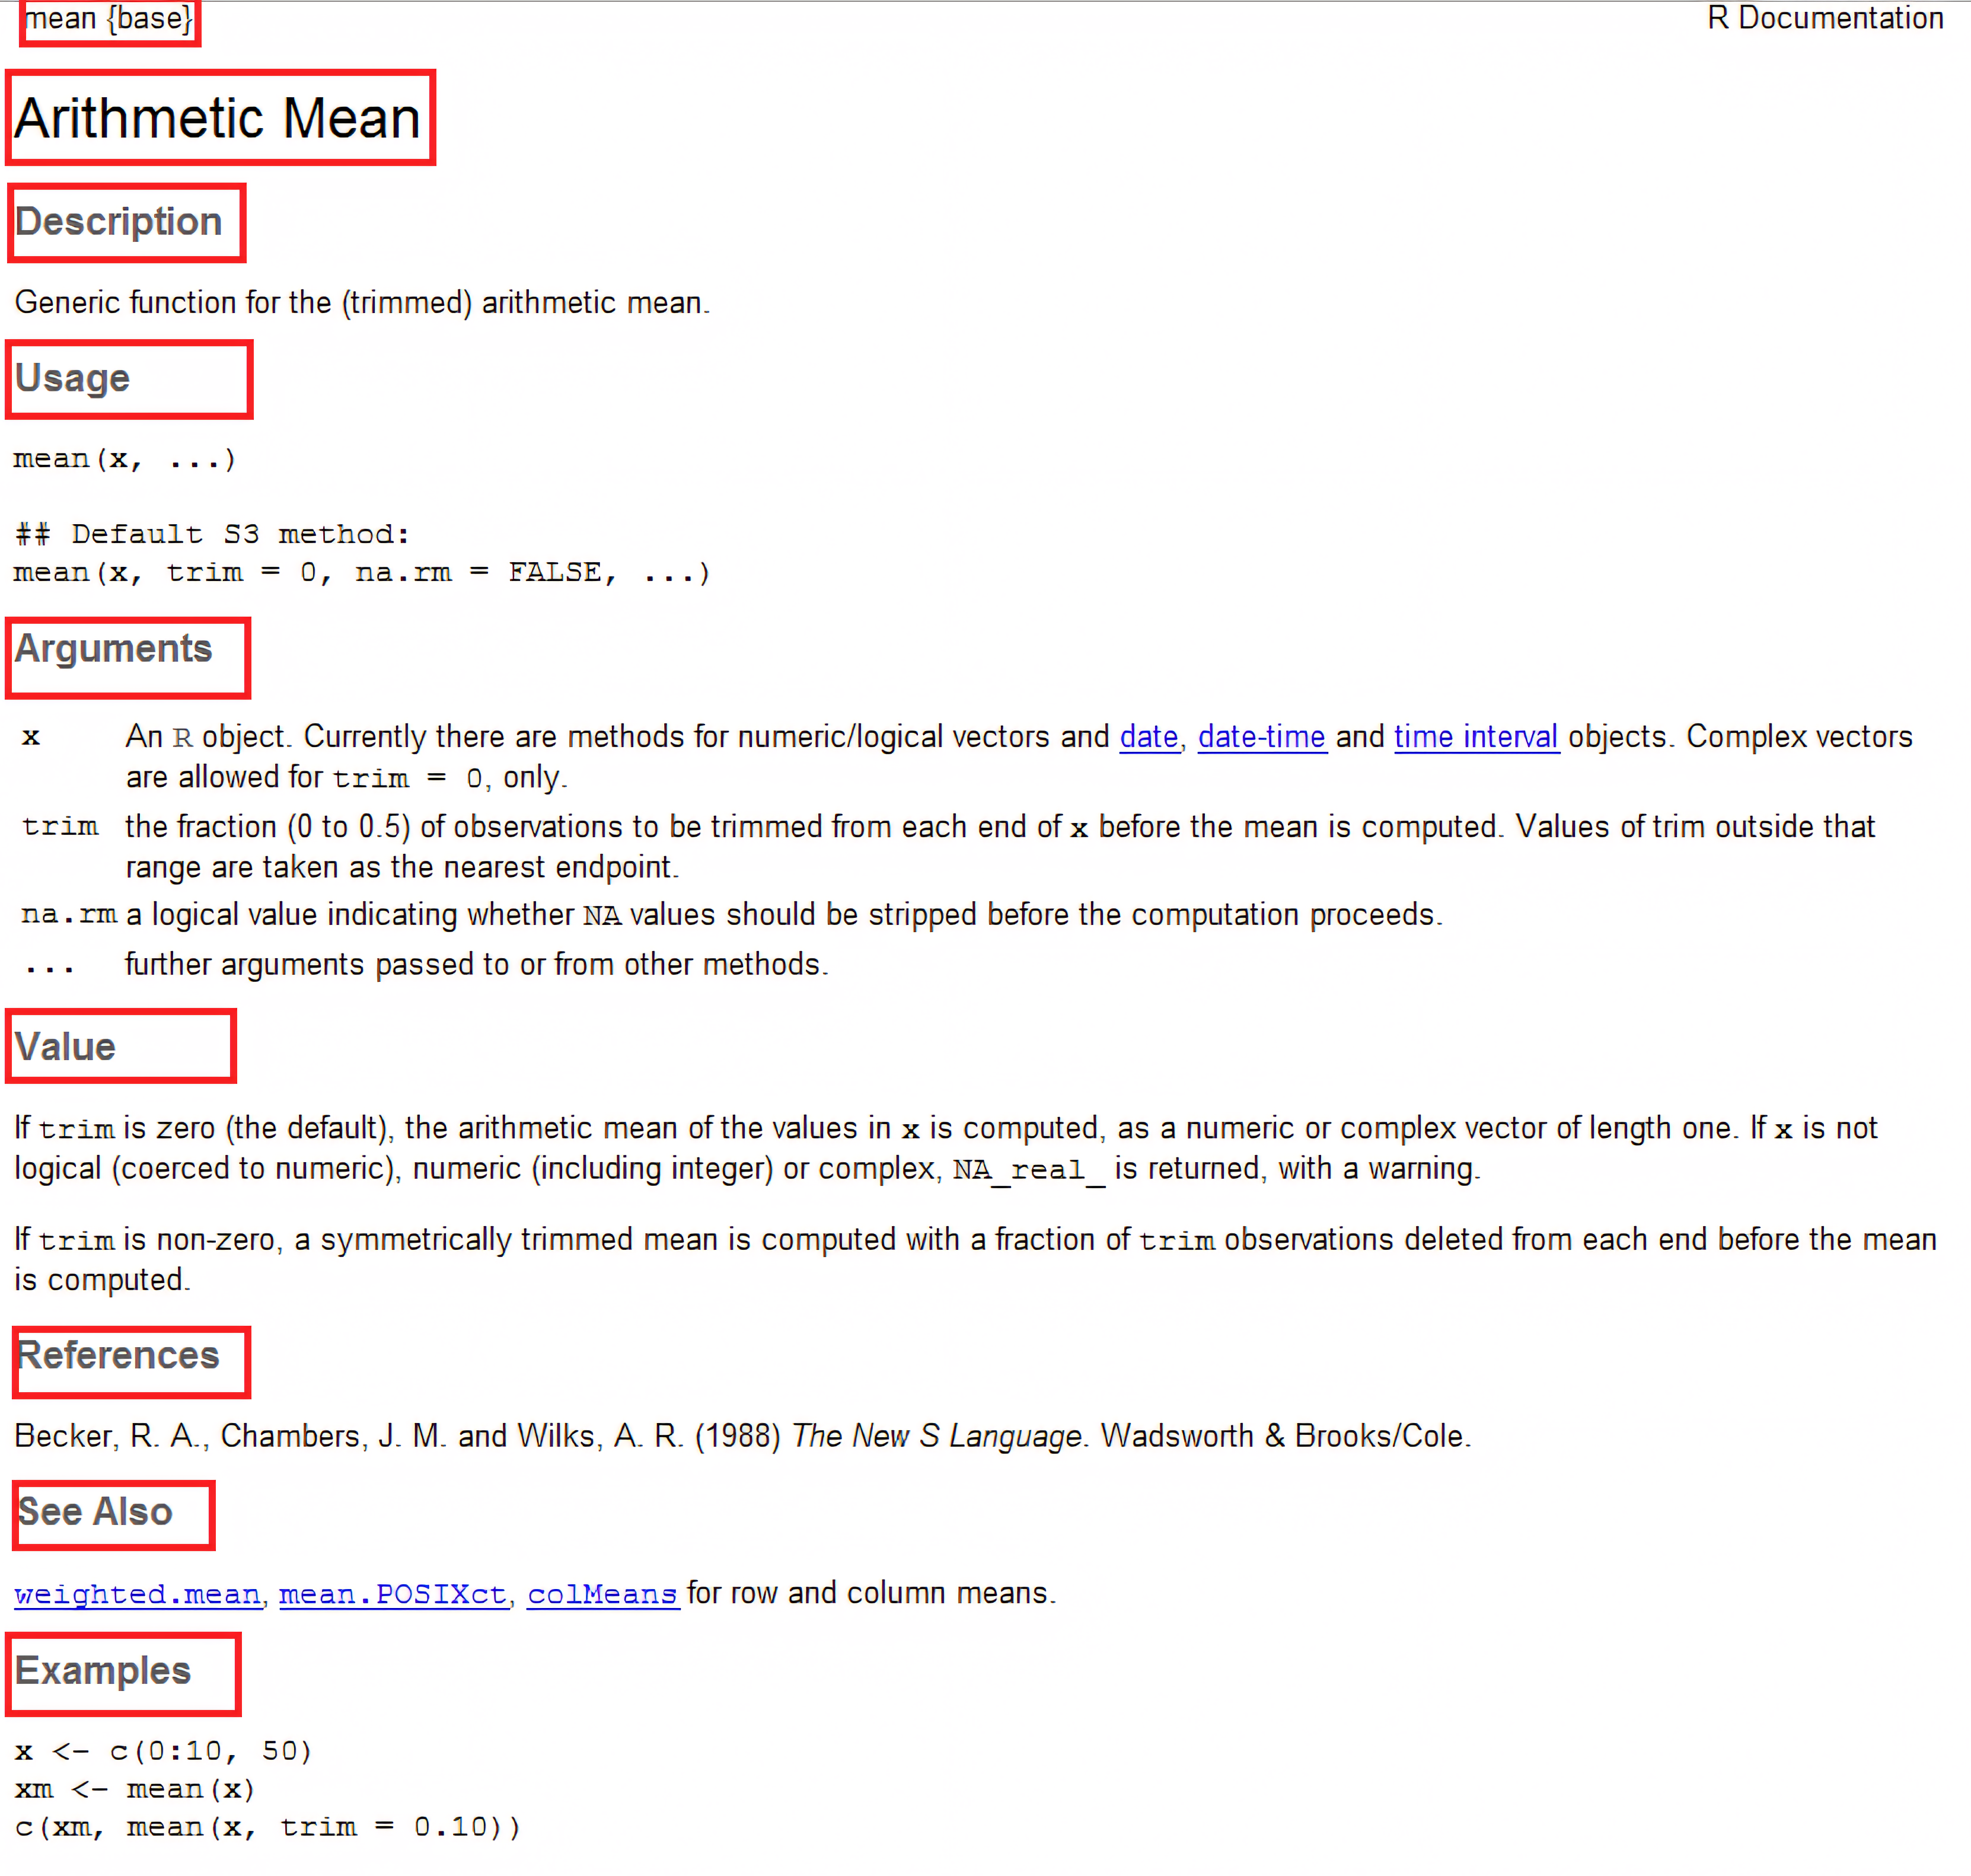
\includegraphics[width=4.6875in,height=4.6875in]{img/r_help.png}
\end{column}

\begin{column}{0.5\textwidth}
\textbf{Description}: descrição da função\\
\textbf{Usage}: uso da função e argumentos\\
\textbf{Arguments}: argumentos e suas especificações\\
\textbf{Details}: detalhes da função\\
\textbf{Value}: interpretar a saída (\emph{output})\\
\textbf{Note}: notas sobre a função\\
\textbf{Authors}: autores da função\\
\textbf{References}: referências bibliográficas da função\\
\textbf{See also}: funções relacionadas\\
\textbf{Examples}: exemplos do uso da função
\end{column}
\end{columns}
\end{block}

\begin{block}{Pacotes}
\protect\hypertarget{pacotes}{}
Conjunto de funções extras para executar tarefas específicas
\end{block}

\begin{block}{Pacotes}
\protect\hypertarget{pacotes-1}{}
Duas fontes

\begin{itemize}
\tightlist
\item
  CRAN (\emph{Comprehensive R Archive Network})
\item
  GitHub (Repositório de códigos)
\end{itemize}

\begin{Shaded}
\begin{Highlighting}[]
\CommentTok{\# numero de pacotes no cran}
\FunctionTok{nrow}\NormalTok{(}\FunctionTok{available.packages}\NormalTok{())}
\end{Highlighting}
\end{Shaded}

\href{https://cran.r-project.org/}{CRAN},
\href{https://www.r-bloggers.com/2017/03/scraping-cran-with-rvest/}{Scraping
CRAN with rvest}
\end{block}

\begin{block}{Pacotes}
\protect\hypertarget{pacotes-2}{}
\textbf{Instalação de pacotes}

\begin{enumerate}
\tightlist
\item
  Download do pacote para o computador (como instalar um software/APP)
\item
  Precisa estar conectado à internet
\item
  O nome do pacote precisa estar entre aspas
\item
  Função (CRAN): \texttt{install.packages("pacote")}
\end{enumerate}

\textbf{Instalar o pacote vegan}

\begin{Shaded}
\begin{Highlighting}[]
\CommentTok{\# instalar pacotes}
\FunctionTok{install.packages}\NormalTok{(}\StringTok{"vegan"}\NormalTok{)}
\end{Highlighting}
\end{Shaded}

\textbf{Verificar pacotes instalados}

\begin{Shaded}
\begin{Highlighting}[]
\CommentTok{\# verificar pacotes instalados}
\FunctionTok{library}\NormalTok{()}
\end{Highlighting}
\end{Shaded}
\end{block}

\begin{block}{Pacotes}
\protect\hypertarget{pacotes-3}{}
\textbf{Carregamento de pacotes}

\begin{enumerate}
\tightlist
\item
  Carregar o pacote para o R (como abrir software/APP)
\item
  Carrega-se toda vez que se abre o R
\item
  Não precisa estar conectado à internet
\item
  O nome do pacote não precisa estar entre aspas
\item
  Funções: \texttt{library(pacote)} ou \texttt{require(pacote)}
\end{enumerate}

\textbf{Carregar o pacote vegan}

\begin{Shaded}
\begin{Highlighting}[]
\CommentTok{\# carregar pacotes}
\FunctionTok{library}\NormalTok{(vegan)}
\end{Highlighting}
\end{Shaded}

\textbf{Verificar pacotes carregados}

\begin{Shaded}
\begin{Highlighting}[]
\CommentTok{\# verificar pacotes carregados}
\FunctionTok{search}\NormalTok{()}
\end{Highlighting}
\end{Shaded}

\begin{verbatim}
 [1] ".GlobalEnv"        "package:vegan"     "package:lattice"  
 [4] "package:permute"   "package:stats"     "package:graphics" 
 [7] "package:grDevices" "package:utils"     "package:datasets" 
[10] "package:methods"   "Autoloads"         "package:base"     
\end{verbatim}
\end{block}
\end{frame}

\begin{frame}{Principais erros}
\protect\hypertarget{principais-erros}{}
\end{frame}

\begin{frame}{Se seu script rodou sem erros, tem algo errado\ldots{}}
\protect\hypertarget{se-seu-script-rodou-sem-erros-tem-algo-errado}{}
\end{frame}

\begin{frame}{}
\protect\hypertarget{section-3}{}
\end{frame}

\begin{frame}{}
\protect\hypertarget{section-4}{}
\end{frame}

\begin{frame}{}
\protect\hypertarget{section-5}{}
\end{frame}

\begin{frame}[fragile]{}
\protect\hypertarget{section-6}{}
Help me help you: um bestiário para entender erros e pedir ajuda no R

\href{https://anotherecoblog.wordpress.com/2020/08/26/help-me-help-you-um-bestiario-para-entender-erros-e-pedir-ajuda-no-r/}{Help
me help you: um bestiário para entender erros e pedir ajuda no R}

\begin{block}{Principais erros}
\protect\hypertarget{principais-erros-1}{}
\textbf{1. Esquecer de completar um código (+)}

Parênteses

\begin{Shaded}
\begin{Highlighting}[]
\FunctionTok{sum}\NormalTok{(}\DecValTok{1}\NormalTok{, }\DecValTok{2}
    \SpecialCharTok{+}
\end{Highlighting}
\end{Shaded}

\begin{verbatim}
Error: <text>:3:0: unexpected end of input
1: sum(1, 2
2:     +
  ^
\end{verbatim}

Aspas

\begin{Shaded}
\begin{Highlighting}[]
\StringTok{"string}
\StringTok{+}
\end{Highlighting}
\end{Shaded}

\begin{verbatim}
Error: <text>:1:1: unexpected INCOMPLETE_STRING
1: "string
2: +
   ^
\end{verbatim}
\end{block}

\begin{block}{Principais erros}
\protect\hypertarget{principais-erros-2}{}
\textbf{2. Esquecer da vírgula}

\begin{Shaded}
\begin{Highlighting}[]
\FunctionTok{sum}\NormalTok{(}\DecValTok{1} \DecValTok{2}\NormalTok{)}
\end{Highlighting}
\end{Shaded}

\begin{verbatim}
Error: <text>:1:7: unexpected numeric constant
1: sum(1 2
          ^
\end{verbatim}

\textbf{3. Chamar um objeto errado}

\begin{Shaded}
\begin{Highlighting}[]
\NormalTok{obj }\OtherTok{\textless{}{-}} \DecValTok{10}
\NormalTok{OBJ}
\end{Highlighting}
\end{Shaded}

\begin{verbatim}
Error in eval(expr, envir, enclos): object 'OBJ' not found
\end{verbatim}
\end{block}

\begin{block}{Principais erros}
\protect\hypertarget{principais-erros-3}{}
\textbf{4. Esquecer de carregar um pacote}

\begin{Shaded}
\begin{Highlighting}[]
\CommentTok{\# carregar dados}
\FunctionTok{data}\NormalTok{(dune)}

\CommentTok{\# funcao do pacote vegan}
\FunctionTok{decostand}\NormalTok{(dune, }\StringTok{"hell"}\NormalTok{)}
\end{Highlighting}
\end{Shaded}

\begin{verbatim}
Error in decostand(dune, "hell"): could not find function "decostand"
\end{verbatim}
\end{block}

\begin{block}{Principais erros}
\protect\hypertarget{principais-erros-4}{}
\textbf{4. Esquecer de carregar um pacote}

\begin{Shaded}
\begin{Highlighting}[]
\CommentTok{\# carregar o pacote}
\FunctionTok{library}\NormalTok{(vegan)}

\DocumentationTok{\#\# carregar dados}
\FunctionTok{data}\NormalTok{(dune)}

\DocumentationTok{\#\# funcao do pacote vegan}
\FunctionTok{decostand}\NormalTok{(dune, }\StringTok{"hell"}\NormalTok{)}
\end{Highlighting}
\end{Shaded}

\begin{verbatim}
    Achimill  Agrostol  Airaprae  Alopgeni  Anthodor  Bellpere  Bromhord
1  0.2357023 0.0000000 0.0000000 0.0000000 0.0000000 0.0000000 0.0000000
2  0.2672612 0.0000000 0.0000000 0.2182179 0.0000000 0.2672612 0.3086067
3  0.0000000 0.3162278 0.0000000 0.4183300 0.0000000 0.2236068 0.0000000
4  0.0000000 0.4216370 0.0000000 0.2108185 0.0000000 0.2108185 0.2581989
5  0.2156655 0.0000000 0.0000000 0.0000000 0.3049971 0.2156655 0.2156655
6  0.2041241 0.0000000 0.0000000 0.0000000 0.2500000 0.0000000 0.0000000
7  0.2236068 0.0000000 0.0000000 0.0000000 0.2236068 0.0000000 0.2236068
8  0.0000000 0.3162278 0.0000000 0.3535534 0.0000000 0.0000000 0.0000000
9  0.0000000 0.2672612 0.0000000 0.2672612 0.0000000 0.0000000 0.0000000
10 0.3049971 0.0000000 0.0000000 0.0000000 0.3049971 0.2156655 0.3049971
11 0.0000000 0.0000000 0.0000000 0.0000000 0.0000000 0.0000000 0.0000000
12 0.0000000 0.3380617 0.0000000 0.4780914 0.0000000 0.0000000 0.0000000
13 0.0000000 0.3892495 0.0000000 0.3892495 0.0000000 0.0000000 0.0000000
14 0.0000000 0.4082483 0.0000000 0.0000000 0.0000000 0.0000000 0.0000000
15 0.0000000 0.4170288 0.0000000 0.0000000 0.0000000 0.0000000 0.0000000
16 0.0000000 0.4605662 0.0000000 0.3481553 0.0000000 0.0000000 0.0000000
17 0.3651484 0.0000000 0.3651484 0.0000000 0.5163978 0.0000000 0.0000000
18 0.0000000 0.0000000 0.0000000 0.0000000 0.0000000 0.2721655 0.0000000
19 0.0000000 0.0000000 0.3110855 0.0000000 0.3592106 0.0000000 0.0000000
20 0.0000000 0.4016097 0.0000000 0.0000000 0.0000000 0.0000000 0.0000000
    Chenalbu  Cirsarve  Comapalu  Eleopalu  Elymrepe  Empenigr  Hyporadi
1  0.0000000 0.0000000 0.0000000 0.0000000 0.4714045 0.0000000 0.0000000
2  0.0000000 0.0000000 0.0000000 0.0000000 0.3086067 0.0000000 0.0000000
3  0.0000000 0.0000000 0.0000000 0.0000000 0.3162278 0.0000000 0.0000000
4  0.0000000 0.2108185 0.0000000 0.0000000 0.2981424 0.0000000 0.0000000
5  0.0000000 0.0000000 0.0000000 0.0000000 0.3049971 0.0000000 0.0000000
6  0.0000000 0.0000000 0.0000000 0.0000000 0.0000000 0.0000000 0.0000000
7  0.0000000 0.0000000 0.0000000 0.0000000 0.0000000 0.0000000 0.0000000
8  0.0000000 0.0000000 0.0000000 0.3162278 0.0000000 0.0000000 0.0000000
9  0.0000000 0.0000000 0.0000000 0.0000000 0.3779645 0.0000000 0.0000000
10 0.0000000 0.0000000 0.0000000 0.0000000 0.0000000 0.0000000 0.0000000
11 0.0000000 0.0000000 0.0000000 0.0000000 0.0000000 0.0000000 0.2500000
12 0.0000000 0.0000000 0.0000000 0.0000000 0.0000000 0.0000000 0.0000000
13 0.1740777 0.0000000 0.0000000 0.0000000 0.0000000 0.0000000 0.0000000
14 0.0000000 0.0000000 0.2886751 0.4082483 0.0000000 0.0000000 0.0000000
15 0.0000000 0.0000000 0.2948839 0.4662524 0.0000000 0.0000000 0.0000000
16 0.0000000 0.0000000 0.0000000 0.4923660 0.0000000 0.0000000 0.0000000
17 0.0000000 0.0000000 0.0000000 0.0000000 0.0000000 0.0000000 0.3651484
18 0.0000000 0.0000000 0.0000000 0.0000000 0.0000000 0.0000000 0.0000000
19 0.0000000 0.0000000 0.0000000 0.0000000 0.0000000 0.2540003 0.4016097
20 0.0000000 0.0000000 0.0000000 0.3592106 0.0000000 0.0000000 0.0000000
    Juncarti  Juncbufo  Lolipere  Planlanc   Poaprat   Poatriv  Ranuflam
1  0.0000000 0.0000000 0.6236096 0.0000000 0.4714045 0.3333333 0.0000000
2  0.0000000 0.0000000 0.3450328 0.0000000 0.3086067 0.4082483 0.0000000
3  0.0000000 0.0000000 0.3872983 0.0000000 0.3535534 0.3872983 0.0000000
4  0.0000000 0.0000000 0.3333333 0.0000000 0.2981424 0.3333333 0.0000000
5  0.0000000 0.0000000 0.2156655 0.3409972 0.2156655 0.3735437 0.0000000
6  0.0000000 0.0000000 0.3535534 0.3227486 0.2500000 0.2886751 0.0000000
7  0.0000000 0.2236068 0.3872983 0.3535534 0.3162278 0.3535534 0.0000000
8  0.3162278 0.0000000 0.3162278 0.0000000 0.3162278 0.3162278 0.2236068
9  0.3086067 0.3086067 0.2182179 0.0000000 0.3086067 0.3450328 0.0000000
10 0.0000000 0.0000000 0.3735437 0.2641353 0.3049971 0.3049971 0.0000000
11 0.0000000 0.0000000 0.4677072 0.3061862 0.3535534 0.0000000 0.0000000
12 0.0000000 0.3380617 0.0000000 0.0000000 0.0000000 0.3380617 0.0000000
13 0.0000000 0.3015113 0.0000000 0.0000000 0.2461830 0.5222330 0.2461830
14 0.0000000 0.0000000 0.0000000 0.0000000 0.0000000 0.0000000 0.2886751
15 0.3611576 0.0000000 0.0000000 0.0000000 0.0000000 0.0000000 0.2948839
16 0.3015113 0.0000000 0.0000000 0.0000000 0.0000000 0.2461830 0.2461830
17 0.0000000 0.0000000 0.0000000 0.3651484 0.2581989 0.0000000 0.0000000
18 0.0000000 0.0000000 0.2721655 0.3333333 0.3333333 0.0000000 0.0000000
19 0.0000000 0.0000000 0.0000000 0.0000000 0.0000000 0.0000000 0.0000000
20 0.3592106 0.0000000 0.0000000 0.0000000 0.0000000 0.0000000 0.3592106
    Rumeacet  Sagiproc  Salirepe  Scorautu  Trifprat  Trifrepe  Vicilath
1  0.0000000 0.0000000 0.0000000 0.0000000 0.0000000 0.0000000 0.0000000
2  0.0000000 0.0000000 0.0000000 0.3450328 0.0000000 0.3450328 0.0000000
3  0.0000000 0.0000000 0.0000000 0.2236068 0.0000000 0.2236068 0.0000000
4  0.0000000 0.3333333 0.0000000 0.2108185 0.0000000 0.1490712 0.0000000
5  0.3409972 0.0000000 0.0000000 0.2641353 0.2156655 0.2156655 0.0000000
6  0.3535534 0.0000000 0.0000000 0.2500000 0.3227486 0.3227486 0.0000000
7  0.2738613 0.0000000 0.0000000 0.2738613 0.2236068 0.2236068 0.0000000
8  0.0000000 0.2236068 0.0000000 0.2738613 0.0000000 0.2236068 0.0000000
9  0.2182179 0.2182179 0.0000000 0.2182179 0.0000000 0.2672612 0.0000000
10 0.0000000 0.0000000 0.0000000 0.2641353 0.0000000 0.3735437 0.1524986
11 0.0000000 0.2500000 0.0000000 0.3952847 0.0000000 0.3061862 0.2500000
12 0.2390457 0.3380617 0.0000000 0.2390457 0.0000000 0.2927700 0.0000000
13 0.0000000 0.2461830 0.0000000 0.2461830 0.0000000 0.2461830 0.0000000
14 0.0000000 0.0000000 0.0000000 0.2886751 0.0000000 0.5000000 0.0000000
15 0.0000000 0.0000000 0.0000000 0.2948839 0.0000000 0.2085144 0.0000000
16 0.0000000 0.0000000 0.0000000 0.0000000 0.0000000 0.0000000 0.0000000
17 0.0000000 0.0000000 0.0000000 0.3651484 0.0000000 0.0000000 0.0000000
18 0.0000000 0.0000000 0.3333333 0.4303315 0.0000000 0.2721655 0.1924501
19 0.0000000 0.3110855 0.3110855 0.4399413 0.0000000 0.2540003 0.0000000
20 0.0000000 0.0000000 0.4016097 0.2540003 0.0000000 0.0000000 0.0000000
    Bracruta  Callcusp
1  0.0000000 0.0000000
2  0.0000000 0.0000000
3  0.2236068 0.0000000
4  0.2108185 0.0000000
5  0.2156655 0.0000000
6  0.3535534 0.0000000
7  0.2236068 0.0000000
8  0.2236068 0.0000000
9  0.2182179 0.0000000
10 0.2156655 0.0000000
11 0.3535534 0.0000000
12 0.3380617 0.0000000
13 0.0000000 0.0000000
14 0.0000000 0.4082483
15 0.4170288 0.0000000
16 0.3481553 0.3015113
17 0.0000000 0.0000000
18 0.4714045 0.0000000
19 0.3110855 0.0000000
20 0.3592106 0.3110855
\end{verbatim}
\end{block}

\begin{block}{Principais erros}
\protect\hypertarget{principais-erros-5}{}
\textbf{5. Usar o nome da função de forma errônea}

\begin{Shaded}
\begin{Highlighting}[]
\FunctionTok{colsums}\NormalTok{(dune)}
\end{Highlighting}
\end{Shaded}

\begin{verbatim}
Error in colsums(dune): could not find function "colsums"
\end{verbatim}

\begin{Shaded}
\begin{Highlighting}[]
\FunctionTok{colSums}\NormalTok{(dune)}
\end{Highlighting}
\end{Shaded}

\begin{verbatim}
Achimill Agrostol Airaprae Alopgeni Anthodor Bellpere Bromhord Chenalbu 
      16       48        5       36       21       13       15        1 
Cirsarve Comapalu Eleopalu Elymrepe Empenigr Hyporadi Juncarti Juncbufo 
       2        4       25       26        2        9       18       13 
Lolipere Planlanc  Poaprat  Poatriv Ranuflam Rumeacet Sagiproc Salirepe 
      58       26       48       63       14       18       20       11 
Scorautu Trifprat Trifrepe Vicilath Bracruta Callcusp 
      54        9       47        4       49       10 
\end{verbatim}
\end{block}
\end{frame}

\begin{frame}{Dúvidas?}
\protect\hypertarget{duxfavidas}{}
\end{frame}

\begin{frame}[fragile]{2. Análise exploratória de dados (AED)}
\protect\hypertarget{anuxe1lise-exploratuxf3ria-de-dados-aed}{}
\begin{block}{Dados}
\protect\hypertarget{dados}{}
\begin{longtable}[]{@{}
  >{\centering\arraybackslash}p{(\columnwidth - 10\tabcolsep) * \real{0.1667}}
  >{\centering\arraybackslash}p{(\columnwidth - 10\tabcolsep) * \real{0.3182}}
  >{\centering\arraybackslash}p{(\columnwidth - 10\tabcolsep) * \real{0.1061}}
  >{\centering\arraybackslash}p{(\columnwidth - 10\tabcolsep) * \real{0.1818}}
  >{\centering\arraybackslash}p{(\columnwidth - 10\tabcolsep) * \real{0.1515}}
  >{\centering\arraybackslash}p{(\columnwidth - 10\tabcolsep) * \real{0.0758}}@{}}
\toprule\noalign{}
\begin{minipage}[b]{\linewidth}\centering
id
\end{minipage} & \begin{minipage}[b]{\linewidth}\centering
especie
\end{minipage} & \begin{minipage}[b]{\linewidth}\centering
peso
\end{minipage} & \begin{minipage}[b]{\linewidth}\centering
comp\_corpo
\end{minipage} & \begin{minipage}[b]{\linewidth}\centering
comp\_asa
\end{minipage} & \begin{minipage}[b]{\linewidth}\centering
\ldots{}
\end{minipage} \\
\midrule\noalign{}
\endhead
LECAVE035 & Columbina talpacoti & 40.64 & 158.5 & 90.51 & \ldots{} \\
LECAVE036 & Columbina talpacoti & 41.05 & 149.73 & 89.42 & \ldots{} \\
LECAVE037 & Columbina talpacoti & 43.96 & 147.62 & 89.32 & \ldots{} \\
LECAVE038 & Columbina talpacoti & 48.01 & 153.44 & 90.57 & \ldots{} \\
\ldots{} & \ldots{} & \ldots{} & \ldots{} & \ldots{} & \ldots{} \\
\bottomrule\noalign{}
\end{longtable}
\end{block}

\begin{block}{Variáveis}
\protect\hypertarget{variuxe1veis}{}
Cada coluna dos nossos dados é uma \textbf{variável} (valores variam)

\begin{verbatim}
Rows: 30
Columns: 10
$ id         <chr> "LECAVE035", "LECAVE036", "LECAVE037", "LECAVE038", "LECAVE~
$ especie    <chr> "Columbina talpacoti", "Columbina talpacoti", "Columbina ta~
$ peso       <dbl> 40.64, 41.05, 43.96, 48.01, 43.43, 9.10, 14.20, 11.30, 13.4~
$ comp_corpo <dbl> 158.50, 149.73, 147.62, 153.44, 144.63, 100.19, 104.93, 97.~
$ comp_asa   <dbl> 90.51, 89.42, 89.32, 90.57, 87.42, 58.10, 63.15, 60.84, 55.~
$ com_cauda  <dbl> 67.38, 73.13, 70.69, 71.10, 68.93, 36.14, 39.34, 33.10, 33.~
$ comp_tarso <dbl> 19.06, 20.09, 18.01, 19.64, 17.05, 16.92, 18.50, 18.85, 18.~
$ comp_bico  <dbl> 14.28, 13.78, 12.49, 12.61, 10.31, 10.30, 8.13, 9.68, 8.70,~
$ larg_bico  <dbl> 4.33, 4.73, 3.64, 3.83, 3.74, 5.83, 5.32, 5.48, 5.47, 5.71,~
$ alt_bico   <dbl> 3.65, 4.04, 4.04, 3.74, 3.66, 5.53, 6.27, 7.12, 6.87, 7.40,~
\end{verbatim}
\end{block}

\begin{block}{Medidas-resumo}
\protect\hypertarget{medidas-resumo}{}
\textbf{Medidas de posição}

\begin{itemize}
\item
  \textbf{Moda}: valor mais frequente das observações
\item
  \textbf{Mediana}: valor que divide as observações ordenadas em duas
  partes iguais
\item
  \textbf{Média aritmética}: soma das observações dividida pelo número
  de observações
\item
  \textbf{Outras médias}: ponderada, geométrica e harmônica
\end{itemize}
\end{block}

\begin{block}{Medidas-resumo}
\protect\hypertarget{medidas-resumo-1}{}
\textbf{Medidas de dispersão}

\begin{itemize}
\item
  \textbf{Variância}: medida de quantas observações diferem do valor
  central (média)
\item
  \textbf{Desvio padrão}: raiz quadrada da variância (mantêm a mesma
  unidade de medida)
\item
  \textbf{Erro padrão}: variação da média amostral em relação à média
  populacional (confiabilidade da média amostral)
\end{itemize}
\end{block}

\begin{block}{Tabelas}
\protect\hypertarget{tabelas}{}
\textbf{Tabelas de frequência}

\begin{itemize}
\item
  \textbf{Dados brutos}: conjunto dos valores numéricos coletados na
  pesquisa
\item
  \textbf{Classes}: intervalo de valores contínuos (0 \textbar--- 1)
\item
  \textbf{Frequência absoluta (fi)}: número de vezes que uma observação
  aparece ou pertencente a um intervalo ou classe
\item
  \textbf{Frequência total}: soma de todas as frequências absolutas (fi)
\item
  \textbf{Frequência relativa (fri)}: valor da razão de cada frequência
  absoluta (fi) com a frequência total (somatório de fi)
\item
  \textbf{Frequência acumulada (Fi)}: obtida somando (acumulando) os
  valores da frequência absoluta (fi)
\item
  \textbf{Frequência relativa acumulada (Fri)}: obtida somando
  (acumulando) os valores da frequência relativa (fri)
\end{itemize}
\end{block}

\begin{block}{Tabelas}
\protect\hypertarget{tabelas-1}{}
\textbf{Tabelas de frequência}

\begin{longtable}[]{@{}
  >{\centering\arraybackslash}p{(\columnwidth - 8\tabcolsep) * \real{0.2000}}
  >{\centering\arraybackslash}p{(\columnwidth - 8\tabcolsep) * \real{0.2000}}
  >{\centering\arraybackslash}p{(\columnwidth - 8\tabcolsep) * \real{0.2000}}
  >{\centering\arraybackslash}p{(\columnwidth - 8\tabcolsep) * \real{0.2000}}
  >{\centering\arraybackslash}p{(\columnwidth - 8\tabcolsep) * \real{0.2000}}@{}}
\toprule\noalign{}
\begin{minipage}[b]{\linewidth}\centering
Classes
\end{minipage} & \begin{minipage}[b]{\linewidth}\centering
Freq. absoluta (fi)
\end{minipage} & \begin{minipage}[b]{\linewidth}\centering
Freq. relativa (fri)
\end{minipage} & \begin{minipage}[b]{\linewidth}\centering
Freq. acumulada (Fi)
\end{minipage} & \begin{minipage}[b]{\linewidth}\centering
Freq. relativa acumulada (Fri)
\end{minipage} \\
\midrule\noalign{}
\endhead
0\textbar---1 & 4 & 0.13 & 4 & 0.13 \\
1\textbar---2 & 8 & 0.26 & 12 & 0.39 \\
2\textbar---3 & 12 & 0.39 & 24 & 0.77 \\
3\textbar---4 & 7 & 0.23 & 31 & 1.00 \\
Total & 31 & 1.00 & & \\
\bottomrule\noalign{}
\end{longtable}
\end{block}

\begin{block}{Gráficos}
\protect\hypertarget{gruxe1ficos}{}
\begin{itemize}
\item
  Melhor forma de apresentar, sintetizar, discutir e interpretar seus
  dados
\item
  Necessário em quase todas as análises estatísticas
\item
  Necessário em quase todas as publicações, trabalhos de consultoria,
  TCC, dissertação, tese, etc.
\item
  Existem vários tipos de gráficos para representar os padrões em seus
  dados para diferentes tipos de finalidades
\item
  De forma simplificada, os gráficos são representações dos nossos dados
  tabulares
\end{itemize}
\end{block}

\begin{block}{Como mentir com estatística?}
\protect\hypertarget{como-mentir-com-estatuxedstica}{}
\includegraphics[width=2.8125in,height=4.16667in]{img/cover_mentir_estatistica.jpg}
\includegraphics[width=9.375in,height=4.6875in]{img/como_mentir_est.png}

\href{https://www.intrinseca.com.br/livro/624/}{Heff (2016)},
\href{https://youtu.be/r6d-RBDlc5I}{Como MENTIR com ESTATÍSTICA}
\end{block}

\begin{block}{Elementos de um gráfico}
\protect\hypertarget{elementos-de-um-gruxe1fico}{}
Representações das colunas (eixos) e linhas (elementos)
\end{block}

\begin{block}{Tipos de variáveis}
\protect\hypertarget{tipos-de-variuxe1veis}{}
\includegraphics[width=5.20833in,height=2.60417in]{img/plot_variables.png}

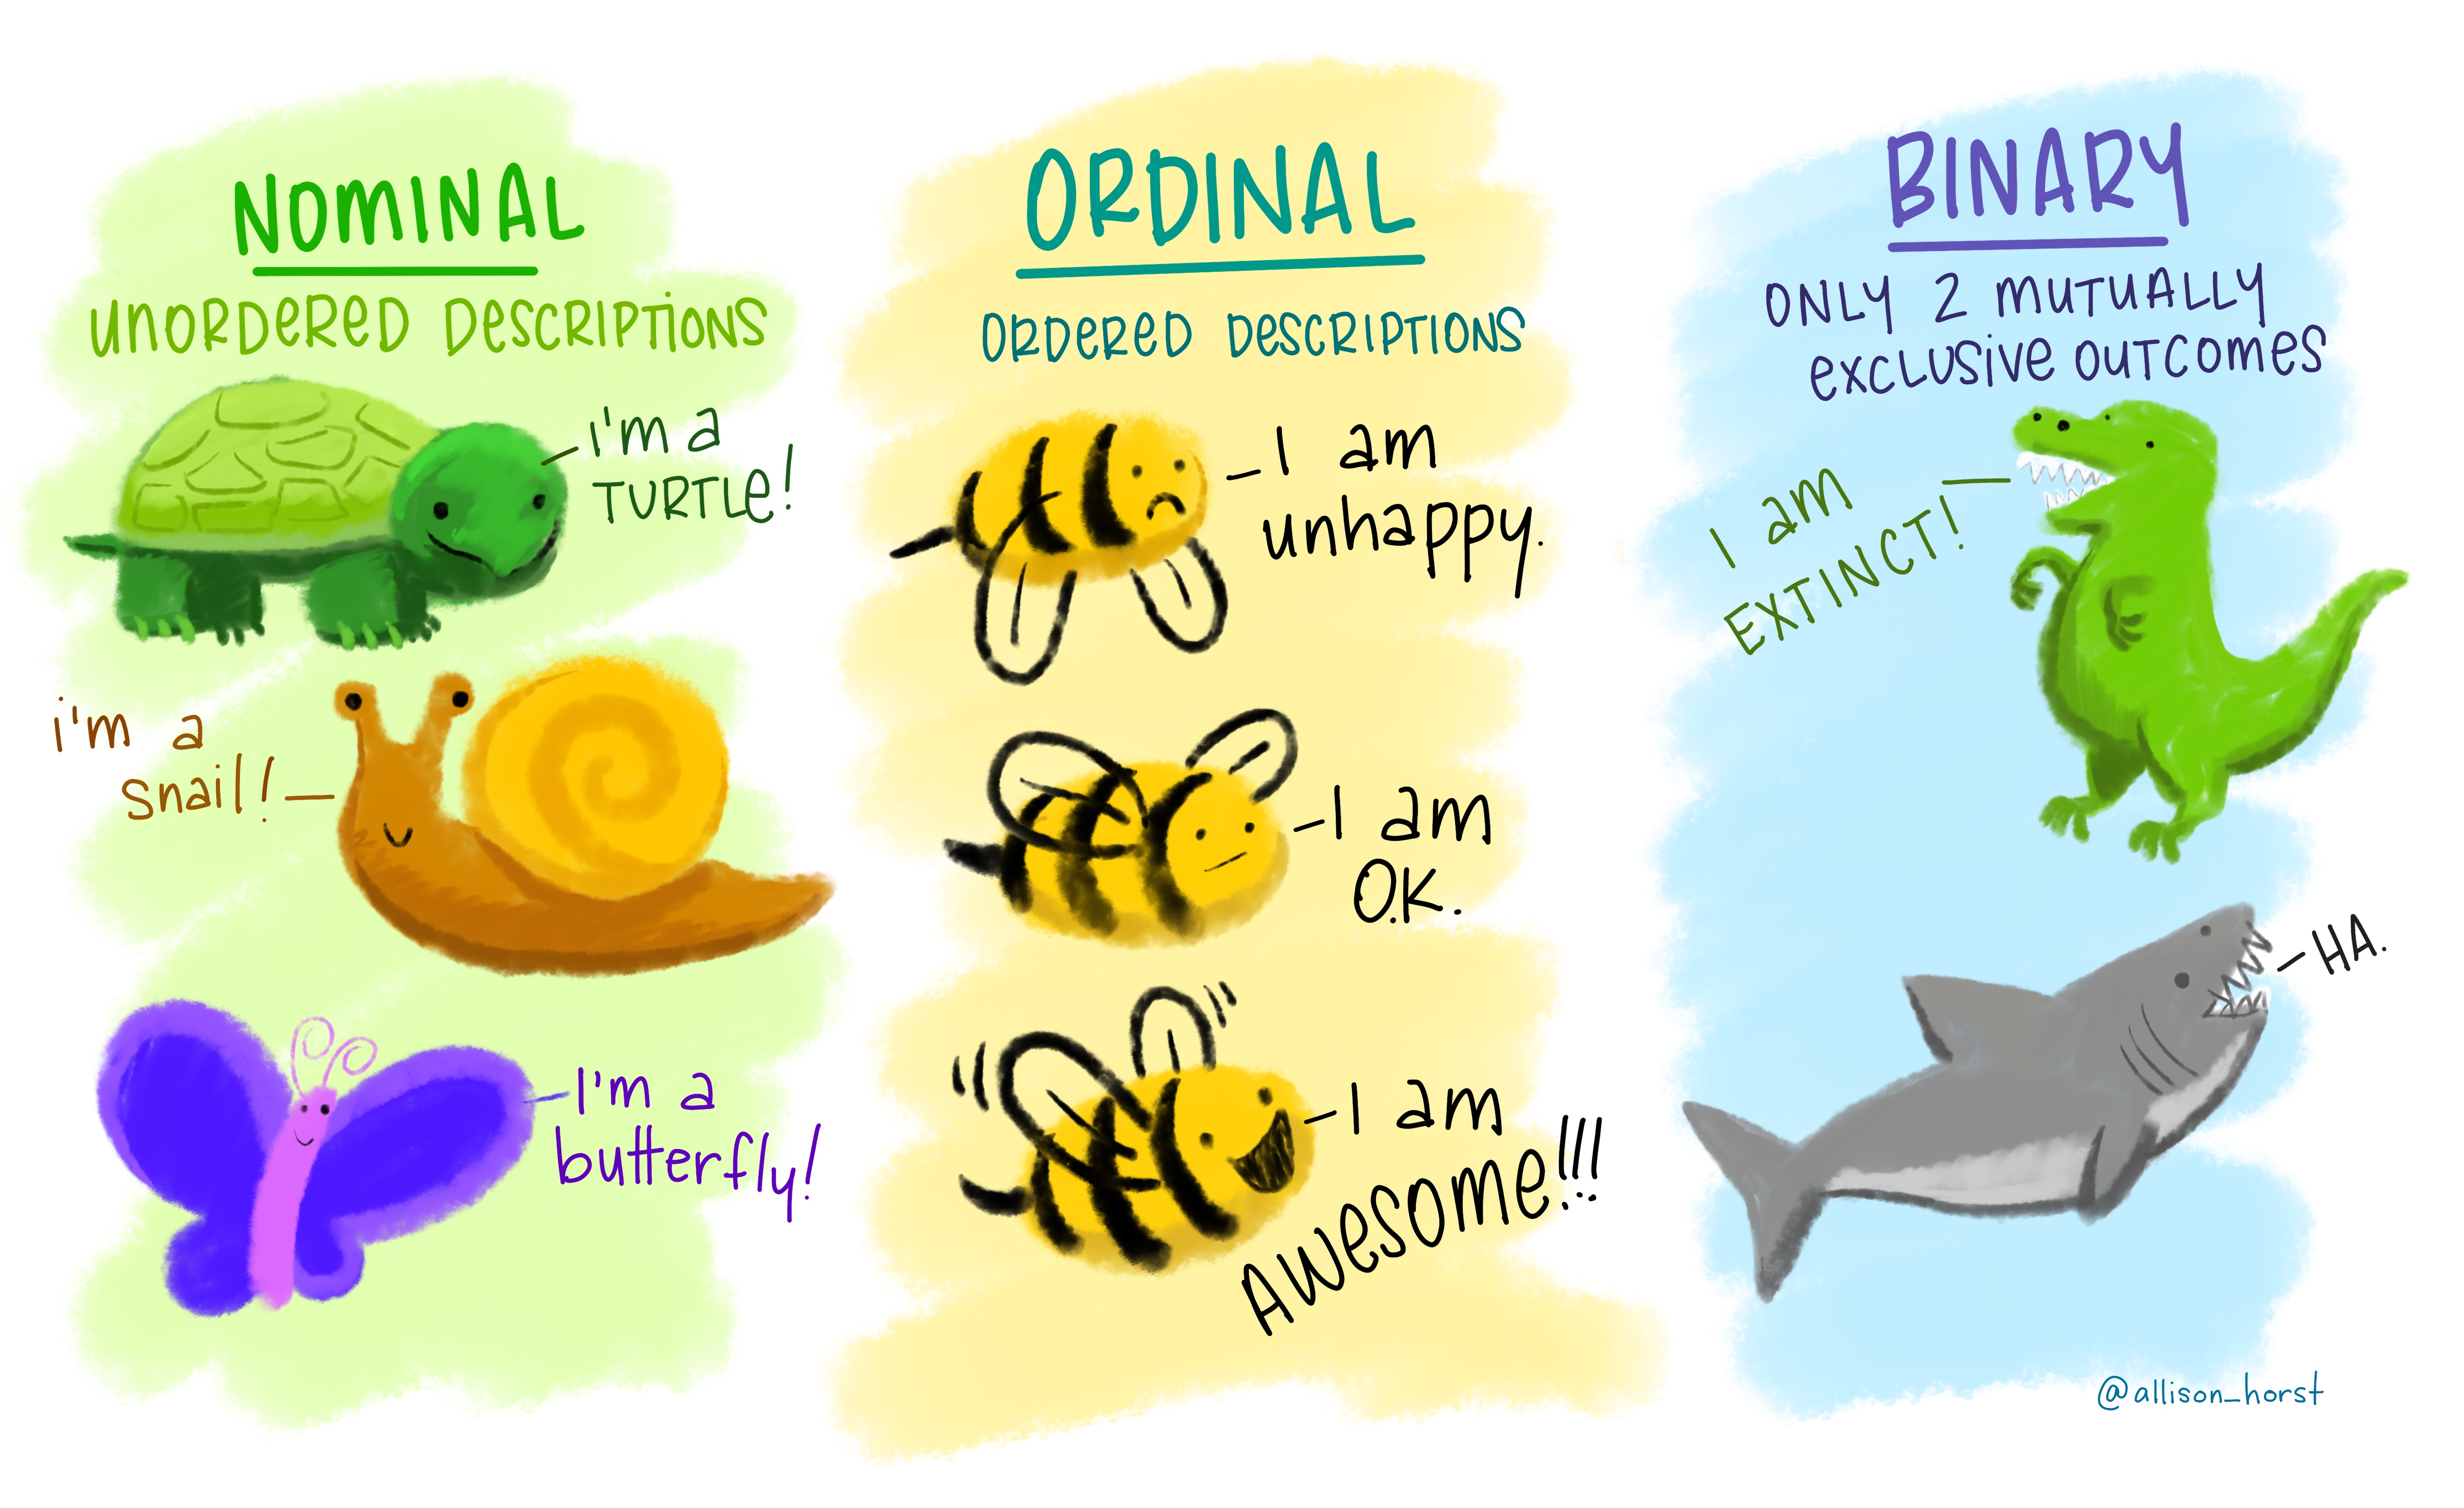
\includegraphics[width=5.20833in,height=3.64583in]{img/nominal_ordinal_binary.png}

\includegraphics[width=5.20833in,height=3.64583in]{img/continuous_discrete_inv.png}

\href{http://greenmaths.st-andrews.ac.uk/}{Matthiopoulos (2011)},
\href{https://twitter.com/allison_horst}{@allison\_horst}
\end{block}

\begin{block}{Tipos de variáveis e tipos gráficos}
\protect\hypertarget{tipos-de-variuxe1veis-e-tipos-gruxe1ficos}{}
\href{https://www.data-to-viz.com/}{from Data to Viz}
\end{block}

\begin{block}{Tipos de variáveis e tipos gráficos}
\protect\hypertarget{tipos-de-variuxe1veis-e-tipos-gruxe1ficos-1}{}
\end{block}

\begin{block}{R CHARTS}
\protect\hypertarget{r-charts}{}
\href{https://r-charts.com/}{R CHARTS}
\end{block}

\begin{block}{Histograma ou densidade}
\protect\hypertarget{histograma-ou-densidade}{}
\begin{itemize}
\item
  Representa dados de uma coluna
\item
  Dados do tipo discreto ou contínuo
\item
  Distribuição de frequência ou densidade
\end{itemize}

\includegraphics[width=3.64583in,height=3.64583in]{img/plot_histogram.png}

\includegraphics[width=3.64583in,height=3.64583in]{img/plot_density.png}

\href{https://www.data-to-viz.com/graph/histogram.html}{histogram},
\href{https://www.data-to-viz.com/graph/density.html}{density}
\end{block}

\begin{block}{Histograma}
\protect\hypertarget{histograma}{}
\pause

\href{https://plotly.com/chart-studio-help/histogram/}{Intro to
Histograms}
\end{block}

\begin{block}{Histograma}
\protect\hypertarget{histograma-1}{}
\href{https://plotly.com/chart-studio-help/histogram/}{Intro to
Histograms}
\end{block}

\begin{block}{Densidade}
\protect\hypertarget{densidade}{}
\href{https://plotly.com/chart-studio-help/histogram/}{Intro to
Histograms}
\end{block}

\begin{block}{Densidade}
\protect\hypertarget{densidade-1}{}
\includegraphics[width=5.72917in,height=3.64583in]{img/hist_fig6.gif}

\pause

\includegraphics[width=5.83333in,height=3.54167in]{img/hist_fig7.gif}

\href{https://plotly.com/chart-studio-help/histogram/}{Intro to
Histograms}
\end{block}

\begin{block}{Gráfico de caixas (\emph{Box plot})}
\protect\hypertarget{gruxe1fico-de-caixas-box-plot}{}
\begin{itemize}
\item
  Representa dados de duas colunas
\item
  Dados do tipo categóricos: X = categórico e Y = contínuo
\item
  Resume informações de medidas contínuas para dois ou mais fatores
  categóricos
\end{itemize}

\includegraphics[width=3.64583in,height=3.64583in]{img/plot_boxplot.png}

\href{https://www.data-to-viz.com/caveat/boxplot.html}{boxplot}
\end{block}

\begin{block}{Gráfico de caixas (\emph{Box plot})}
\protect\hypertarget{gruxe1fico-de-caixas-box-plot-1}{}
\begin{itemize}
\item
  Intervalo inter-quartil (\emph{interquartile range} - IQR)
\item
  Limite inferior e limite superipor (1.5 x IQR)
\item
  Valores exteriores (\emph{outliers})
\end{itemize}

\includegraphics[width=5.20833in,height=2.91667in]{img/plot_boxplot1.png}
\includegraphics[width=4.47917in,height=4.47917in]{img/plot_boxplot2.png}

\href{https://www.kdnuggets.com/2019/11/understanding-boxplots.html}{Understanding
Boxplots}
\end{block}

\begin{block}{Outlier}
\protect\hypertarget{outlier}{}
Observação coletado de forma errônea ou devido à arredondamentos
\end{block}

\begin{block}{Gráfico de caixas (\emph{Box plot})}
\protect\hypertarget{gruxe1fico-de-caixas-box-plot-2}{}
\pause

\href{https://plotly.com/chart-studio-help/what-is-a-box-plot/}{Intro to
Box Plots}
\end{block}

\begin{block}{Gráfico de caixas (\emph{Box plot})}
\protect\hypertarget{gruxe1fico-de-caixas-box-plot-3}{}
\pause

\href{https://plotly.com/chart-studio-help/what-is-a-box-plot/}{Intro to
Box Plots}
\end{block}

\begin{block}{Gráfico de caixas (\emph{Box plot})}
\protect\hypertarget{gruxe1fico-de-caixas-box-plot-4}{}
\pause

\includegraphics[width=10.41667in,height=3.64583in]{img/boxplotfig7.gif}

\href{https://plotly.com/chart-studio-help/what-is-a-box-plot/}{Intro to
Box Plots}
\end{block}

\begin{block}{Gráfico de caixas (\emph{Box plot})}
\protect\hypertarget{gruxe1fico-de-caixas-box-plot-5}{}
\href{https://plotly.com/chart-studio-help/what-is-a-box-plot/}{Intro to
Box Plots}
\end{block}

\begin{block}{Gráfico de caixas (\emph{Box plot})}
\protect\hypertarget{gruxe1fico-de-caixas-box-plot-6}{}
\href{https://plotly.com/chart-studio-help/what-is-a-box-plot/}{Intro to
Box Plots}
\end{block}
\end{frame}

\begin{frame}{3. Análise de dados multivariados}
\protect\hypertarget{anuxe1lise-de-dados-multivariados}{}
\begin{block}{Dados em matrizes}
\protect\hypertarget{dados-em-matrizes}{}
\href{https://www.fbbva.es/microsite/multivariate-statistics/}{Greenacre
\& Primicerio (2013)}
\end{block}

\begin{block}{Objetos e descritores}
\protect\hypertarget{objetos-e-descritores}{}
\begin{itemize}
\tightlist
\item
  \textbf{Objetos (1)}: linhas - representam os locais ou indivíduos
  amostrados
\item
  \textbf{Descritores (2)}: colunas - representam as variáveis
  mensuradas ou contagens
\end{itemize}

\href{https://www.fbbva.es/microsite/multivariate-statistics/}{Greenacre
\& Primicerio (2013)}
\end{block}

\begin{block}{Análises no modo R e Q}
\protect\hypertarget{anuxe1lises-no-modo-r-e-q}{}
\begin{itemize}
\tightlist
\item
  \textbf{Modo R}: análise da relação dos descritores (correlação e
  covariância)
\item
  \textbf{Modo Q}: análise da relação dos objetos (distância ou
  associação)
\end{itemize}

\href{https://www.fbbva.es/microsite/multivariate-statistics/}{Greenacre
\& Primicerio (2013)}
\end{block}

\begin{block}{Tipos de análises multivariadas}
\protect\hypertarget{tipos-de-anuxe1lises-multivariadas}{}
\begin{columns}[T]
\begin{column}{0.5\textwidth}
\begin{itemize}
\tightlist
\item
  \textbf{Agrupamento}: agrupar objetos mais semelhantes entre si
\end{itemize}
\end{column}

\begin{column}{0.5\textwidth}
\begin{itemize}
\item
  \textbf{Ordenação}: ordenar objetos num espaço com menos dimensões
\end{itemize}
\end{column}
\end{columns}

\href{https://www.fbbva.es/microsite/multivariate-statistics/}{Greenacre
\& Primicerio (2013)}
\end{block}
\end{frame}

\begin{frame}{Mas antes, vamos entender o que medimos e ajustes prévios
dos dados}
\protect\hypertarget{mas-antes-vamos-entender-o-que-medimos-e-ajustes-pruxe9vios-dos-dados}{}
\begin{block}{Escala de medidas}
\protect\hypertarget{escala-de-medidas}{}
\begin{itemize}
\tightlist
\item
  \textbf{Nominal}: nomes sem ordem (1. pelágico ou 2. litoral)
\item
  \textbf{Ordinal}: nomes com ordem (1. argila, 2. silte, 3. areia, 4.
  cascalho ou 5. pedra)
\item
  \textbf{Razão}: medidas multiplicativas (biomassa, concentração,
  comprimento)
\item
  \textbf{Intervalo}: medidas adicionais (tempo, temperatura)
\item
  \textbf{Contagem}: enumeração (abundância)
\item
  \textbf{Composição}: proporções que somam um (areia, silte e argila)
\end{itemize}

\href{https://www.fbbva.es/microsite/multivariate-statistics/}{Greenacre
\& Primicerio (2013)}
\end{block}

\begin{block}{Escala de medidas (unidades)}
\protect\hypertarget{escala-de-medidas-unidades}{}
\begin{itemize}
\item
  Variáveis ambientais geralmente são medidas em diferentes unidades
\item
  Essa diferença deve ser considera quando realizamos análises
  multivariadas
\item
  Ex.: temperatura (ºC), distância da margem (m), área (m²), volume (m³)
\end{itemize}

\href{https://www.fbbva.es/microsite/multivariate-statistics/}{Greenacre
\& Primicerio (2013)}
\end{block}

\begin{block}{Transformação (\emph{Transformation})}
\protect\hypertarget{transformauxe7uxe3o-transformation}{}
Muda a escala de variação ou natureza da variável

\begin{itemize}
\tightlist
\item
  \textbf{Logaritmo}: muda a escala dos valores
\end{itemize}

\[x' = log_{10}(100) = 2\]

\href{https://www.fbbva.es/microsite/multivariate-statistics/}{Greenacre
\& Primicerio (2013)}
\end{block}

\begin{block}{Transformação (\emph{Transformation})}
\protect\hypertarget{transformauxe7uxe3o-transformation-1}{}
Muda a escala de variação ou natureza da variável

\begin{itemize}
\tightlist
\item
  \textbf{Box-Cox}: transformações usando potências (λ)
\end{itemize}

\[x' = \frac{1}{\lambda}(x^\lambda - 1)\]

\href{https://www.fbbva.es/microsite/multivariate-statistics/}{Greenacre
\& Primicerio (2013)}
\end{block}

\begin{block}{Transformação (\emph{Transformation})}
\protect\hypertarget{transformauxe7uxe3o-transformation-2}{}
Muda a escala de variação ou natureza da variável

\begin{itemize}
\tightlist
\item
  \textbf{Dummy}: variáveis categóricas são codificadas como
  \emph{variáveis dummy} (0 e 1)
\end{itemize}

\begin{longtable}[]{@{}ccc@{}}
\toprule\noalign{}
classe & dummy1 & dummy2 \\
\midrule\noalign{}
\endhead
floresta & 0 & 0 \\
silvicultura & 1 & 0 \\
pastagem & 0 & 1 \\
\bottomrule\noalign{}
\end{longtable}

\href{https://www.fbbva.es/microsite/multivariate-statistics/}{Greenacre
\& Primicerio (2013)}
\end{block}

\begin{block}{Transformação (\emph{Transformation})}
\protect\hypertarget{transformauxe7uxe3o-transformation-3}{}
Muda a escala de variação ou natureza da variável

\begin{itemize}
\tightlist
\item
  \textbf{Dummy}: variáveis categóricas são codificadas como
  \emph{variáveis dummy} (0 e 1)
\end{itemize}

\begin{longtable}[]{@{}cccc@{}}
\toprule\noalign{}
classe & dummy1 & dummy2 & dummy3 \\
\midrule\noalign{}
\endhead
floresta & 0 & 0 & 0 \\
silvicultura & 1 & 0 & 0 \\
pastagem & 0 & 1 & 0 \\
cana & 0 & 0 & 1 \\
\bottomrule\noalign{}
\end{longtable}

\href{https://www.fbbva.es/microsite/multivariate-statistics/}{Greenacre
\& Primicerio (2013)}
\end{block}

\begin{block}{Transformação (\emph{Transformation})}
\protect\hypertarget{transformauxe7uxe3o-transformation-4}{}
Muda a escala de variação ou natureza da variável

\begin{itemize}
\tightlist
\item
  \textbf{Fuzzy}: variáveis contínuas são codificadas como
  \emph{variáveis fuzzy} (``baixo'', ``médio'' e ``alto)
\end{itemize}

\href{https://www.fbbva.es/microsite/multivariate-statistics/}{Greenacre
\& Primicerio (2013)}
\end{block}

\begin{block}{Padronização (\emph{Standardization})}
\protect\hypertarget{padronizauxe7uxe3o-standardization}{}
Centralização das variáveis para terem a mesma variação

\href{https://www.fbbva.es/microsite/multivariate-statistics/}{Greenacre
\& Primicerio (2013)}
\end{block}

\begin{block}{Padronização (\emph{Standardization})}
\protect\hypertarget{padronizauxe7uxe3o-standardization-1}{}
\textbf{Z-Score}: média = 0 e desvio padrão = 1

\href{https://www.fbbva.es/microsite/multivariate-statistics/}{Greenacre
\& Primicerio (2013)}
\end{block}

\begin{block}{Padronização (\emph{Standardization})}
\protect\hypertarget{padronizauxe7uxe3o-standardization-2}{}
\begin{itemize}
\tightlist
\item
  valor padronizado = (valor original -- media) / desvio padrao
\end{itemize}

\begin{columns}[T]
\begin{column}{0.5\textwidth}
\end{column}

\begin{column}{0.5\textwidth}
\end{column}
\end{columns}

\href{https://www.fbbva.es/microsite/multivariate-statistics/}{Greenacre
\& Primicerio (2013)}
\end{block}
\end{frame}

\begin{frame}{Com os dados ajustados, vamos calcular medidas entre os
objetos}
\protect\hypertarget{com-os-dados-ajustados-vamos-calcular-medidas-entre-os-objetos}{}
\begin{block}{Medidas entre objetos}
\protect\hypertarget{medidas-entre-objetos}{}
Medidas ou índices podem ser:

\begin{enumerate}
\tightlist
\item
  \textbf{Medidas de distância}: aplicadas a dados quantitativos e não
  possuem limites superiores (dependem da unidade de medida)
\end{enumerate}

\begin{itemize}
\tightlist
\item
  Valores de distância (d): 0 (idênticos) a ∞ (diferentes)
\end{itemize}

\pause

\begin{enumerate}
\setcounter{enumi}{1}
\tightlist
\item
  \textbf{Medidas de associação}: aplicadas a diversos tipos de dados
  (qualitativos ou quantitativos) e possuem limite superior
  (similaridade é máxima (S=1) quando dois objetos são idênticos)
\end{enumerate}

\begin{itemize}
\item
  Valores de similaridade (S): 0 (diferentes) a 1 (idênticos)
\item
  Valores de dissimilaridade (D): 0 (idênticos) a 1 (diferentes)
\end{itemize}

\[D = 1 - S\]

\href{http://www.numericalecology.com/indexen.html}{Legendre \& Legendre
(2012)}
\end{block}

\begin{block}{Medidas de distância}
\protect\hypertarget{medidas-de-distuxe2ncia}{}
\textbf{Distância Euclidiana} (Dados ambientais)

\begin{columns}[T]
\begin{column}{0.35\textwidth}
\end{column}

\begin{column}{0.65\textwidth}
\end{column}
\end{columns}

\href{https://www.fbbva.es/microsite/multivariate-statistics/}{Greenacre
\& Primicerio (2013)}
\end{block}

\begin{block}{Medidas de distância}
\protect\hypertarget{medidas-de-distuxe2ncia-1}{}
\textbf{Distância Euclidiana} (Dados ambientais)

\begin{columns}[T]
\begin{column}{0.35\textwidth}
\end{column}

\begin{column}{0.65\textwidth}
\end{column}
\end{columns}

\href{https://www.fbbva.es/microsite/multivariate-statistics/}{Greenacre
\& Primicerio (2013)}
\end{block}

\begin{block}{Medidas de distância}
\protect\hypertarget{medidas-de-distuxe2ncia-2}{}
\textbf{Distância Euclidiana} (Dados ambientais)

\begin{columns}[T]
\begin{column}{0.35\textwidth}
\end{column}

\begin{column}{0.65\textwidth}
\end{column}
\end{columns}

\href{https://www.fbbva.es/microsite/multivariate-statistics/}{Greenacre
\& Primicerio (2013)}
\end{block}

\begin{block}{Medidas de distância}
\protect\hypertarget{medidas-de-distuxe2ncia-3}{}
\textbf{Distância Euclidiana} (Dados ambientais)

\[d_{x,y} = \sqrt{(x_1 - y_1)^2 + (x_2 - y_2)^2}\]
\[d_{x,y} = \sqrt{(x_1 - y_1)^2 + (x_2 - y_2)^2 + (x_3 - y_3)^2}\]
\[d_{x,y} = \sqrt{\sum_{j=1}^{J}(x_j - y_j)^2}\]

\href{https://www.fbbva.es/microsite/multivariate-statistics/}{Greenacre
\& Primicerio (2013)}
\end{block}

\begin{block}{Medidas de distância}
\protect\hypertarget{medidas-de-distuxe2ncia-4}{}
\textbf{Distância Euclidiana} (Dados ambientais)

\begin{itemize}
\tightlist
\item
  Sem padronização
\end{itemize}

\[d_{s29,s30} = \sqrt{(51 - 90)^2 + (6.0 - 1.9)^2 + (3.0 - 2.9)^2} = 48.17\]

\begin{itemize}
\tightlist
\item
  Com padronização
\end{itemize}

\[d_{s29,s30} = \sqrt{(-1.5 - 1.6)^2 + (.7 - (-1.2))^2 + (-.2 - (-.6))^2} = 3.6\]

\href{https://www.fbbva.es/microsite/multivariate-statistics/}{Greenacre
\& Primicerio (2013)}
\end{block}
\end{frame}

\begin{frame}{Com as distâncias entre objetos calculadas, vamos
relacionar esses objetos}
\protect\hypertarget{com-as-distuxe2ncias-entre-objetos-calculadas-vamos-relacionar-esses-objetos}{}
\begin{block}{Medidas de distância}
\protect\hypertarget{medidas-de-distuxe2ncia-5}{}
\textbf{Matriz de distântica Euclidiana}

\href{https://www.fbbva.es/microsite/multivariate-statistics/}{Greenacre
\& Primicerio (2013)}
\end{block}

\begin{block}{Medidas de associação}
\protect\hypertarget{medidas-de-associauxe7uxe3o}{}
\textbf{Dissimilaridade de Bray-Curtis} (Abundância de espécies)

\[b_{i,i'} = \frac{\sum_{j = 1}^{J}{|n_{ij} - n_{i'j}|}}{n_{i+} + n_{i'+}}\]
\[b_{s29,s30} = \frac{|11 - 24| + |0 - 37| + |7 - 5| + |8 - 18| + |0 - 1|}{26 + 85} = 0.568\]

\href{https://www.fbbva.es/microsite/multivariate-statistics/}{Greenacre
\& Primicerio (2013)}
\end{block}

\begin{block}{Medidas de associação}
\protect\hypertarget{medidas-de-associauxe7uxe3o-1}{}
\textbf{Matriz de dissimilaridade de Bray-Curtis}

\href{https://www.fbbva.es/microsite/multivariate-statistics/}{Greenacre
\& Primicerio (2013)}
\end{block}

\begin{block}{Medidas de associação}
\protect\hypertarget{medidas-de-associauxe7uxe3o-2}{}
\textbf{Dissimilaridade de Jaccard} (Indidência de espécies)

\href{https://www.fbbva.es/microsite/multivariate-statistics/}{Greenacre
\& Primicerio (2013)}
\end{block}

\begin{block}{Medidas de associação}
\protect\hypertarget{medidas-de-associauxe7uxe3o-3}{}
\textbf{Dissimilaridade de Jaccard} (Indidência de espécies)

\[j_{ii'} = 1 - \frac{a}{a + b + c}\] Onde:

a = número de espécies compartilhadas

b = número de espécies exclusivas do local 1

c = número de espécies exclusivas do local 2

\href{https://www.fbbva.es/microsite/multivariate-statistics/}{Greenacre
\& Primicerio (2013)}
\end{block}

\begin{block}{Medidas de associação}
\protect\hypertarget{medidas-de-associauxe7uxe3o-4}{}
\textbf{Dissimilaridade de Jaccard} (Indidência de espécies)

\[j_{ii'} = 1 - \frac{a}{a + b + c}\]
\[j_{AB} = 1 - \frac{4}{4 + 3 + 1} = 0.5\]

\href{https://www.fbbva.es/microsite/multivariate-statistics/}{Greenacre
\& Primicerio (2013)}
\end{block}

\begin{block}{Medidas de associação}
\protect\hypertarget{medidas-de-associauxe7uxe3o-5}{}
\textbf{Matriz de dissimilaridade de Jaccard}

\href{https://www.fbbva.es/microsite/multivariate-statistics/}{Greenacre
\& Primicerio (2013)}
\end{block}

\begin{block}{Tipos de análises multivariadas}
\protect\hypertarget{tipos-de-anuxe1lises-multivariadas-1}{}
\begin{columns}[T]
\begin{column}{0.5\textwidth}
\begin{itemize}
\tightlist
\item
  \textbf{Agrupamento}: agrupar objetos mais semelhantes entre si
\end{itemize}
\end{column}

\begin{column}{0.5\textwidth}
\begin{itemize}
\item
  \textbf{Ordenação}: ordenar objetos num espaço com menos dimensões
\end{itemize}
\end{column}
\end{columns}

\href{https://www.fbbva.es/microsite/multivariate-statistics/}{Greenacre
\& Primicerio (2013)}
\end{block}

\begin{block}{Tipos de análises de agrupamento}
\protect\hypertarget{tipos-de-anuxe1lises-de-agrupamento}{}
\begin{columns}[T]
\begin{column}{0.5\textwidth}
\begin{itemize}
\tightlist
\item
  \textbf{Hierárquico}: objetos de um grupo se tornam elementos do grupo
  superior
\end{itemize}
\end{column}

\begin{column}{0.5\textwidth}
\begin{itemize}
\item
  \textbf{Não-hierárquico}: define-se k grupos e aloca-se os objetos aos
  grupos
\end{itemize}
\end{column}
\end{columns}

\href{https://www.fbbva.es/microsite/multivariate-statistics/}{Greenacre
\& Primicerio (2013)}
\end{block}

\begin{block}{Análises de agrupamento (\emph{Cluster})}
\protect\hypertarget{anuxe1lises-de-agrupamento-cluster}{}
\textbf{1. Pares mais parecidos (menor dissimilaridade) = (B,F)}

\begin{columns}[T]
\begin{column}{0.65\textwidth}
\end{column}

\begin{column}{0.35\textwidth}
\end{column}
\end{columns}

\href{https://www.fbbva.es/microsite/multivariate-statistics/}{Greenacre
\& Primicerio (2013)}
\end{block}

\begin{block}{Análises de agrupamento (\emph{Cluster})}
\protect\hypertarget{anuxe1lises-de-agrupamento-cluster-1}{}
\textbf{2. Recalcular a distância do grupo (B,F) para os demais}

\href{https://www.fbbva.es/microsite/multivariate-statistics/}{Greenacre
\& Primicerio (2013)}
\end{block}

\begin{block}{Análises de agrupamento (\emph{Cluster})}
\protect\hypertarget{anuxe1lises-de-agrupamento-cluster-2}{}
\textbf{3. Pares mais parecidos (menor dissimilaridade) = (A,E)}

\begin{columns}[T]
\begin{column}{0.65\textwidth}
\end{column}

\begin{column}{0.35\textwidth}
\end{column}
\end{columns}

\href{https://www.fbbva.es/microsite/multivariate-statistics/}{Greenacre
\& Primicerio (2013)}
\end{block}

\begin{block}{Análises de agrupamento (\emph{Cluster})}
\protect\hypertarget{anuxe1lises-de-agrupamento-cluster-3}{}
\textbf{4. Recalcular a distância do grupo (A,E) para os demais}

\href{https://www.fbbva.es/microsite/multivariate-statistics/}{Greenacre
\& Primicerio (2013)}
\end{block}

\begin{block}{Análises de agrupamento (\emph{Cluster})}
\protect\hypertarget{anuxe1lises-de-agrupamento-cluster-4}{}
\textbf{5. Pares mais parecidos (menor dissimilaridade) = (C,G)}

\begin{columns}[T]
\begin{column}{0.65\textwidth}
\end{column}

\begin{column}{0.35\textwidth}
\end{column}
\end{columns}

\href{https://www.fbbva.es/microsite/multivariate-statistics/}{Greenacre
\& Primicerio (2013)}
\end{block}

\begin{block}{Análises de agrupamento (\emph{Cluster})}
\protect\hypertarget{anuxe1lises-de-agrupamento-cluster-5}{}
\textbf{6. Recalcular a distância do grupo (C,G) para os demais}

\href{https://www.fbbva.es/microsite/multivariate-statistics/}{Greenacre
\& Primicerio (2013)}
\end{block}

\begin{block}{Análises de agrupamento (\emph{Cluster})}
\protect\hypertarget{anuxe1lises-de-agrupamento-cluster-6}{}
\textbf{7. Pares mais parecidos (menor dissimilaridade) = (A,E),(C,G)}

\begin{columns}[T]
\begin{column}{0.65\textwidth}
\end{column}

\begin{column}{0.35\textwidth}
\end{column}
\end{columns}

\href{https://www.fbbva.es/microsite/multivariate-statistics/}{Greenacre
\& Primicerio (2013)}
\end{block}

\begin{block}{Análises de agrupamento (\emph{Cluster})}
\protect\hypertarget{anuxe1lises-de-agrupamento-cluster-7}{}
\textbf{8. Recalcular a distância do grupo (A,E,C,G) para os demais}

\href{https://www.fbbva.es/microsite/multivariate-statistics/}{Greenacre
\& Primicerio (2013)}
\end{block}

\begin{block}{Análises de agrupamento (\emph{Cluster})}
\protect\hypertarget{anuxe1lises-de-agrupamento-cluster-8}{}
\textbf{9. Pares mais parecidos (menor dissim.) = (A,E,C,G),(B,F)}

\begin{columns}[T]
\begin{column}{0.65\textwidth}
\end{column}

\begin{column}{0.35\textwidth}
\end{column}
\end{columns}

\href{https://www.fbbva.es/microsite/multivariate-statistics/}{Greenacre
\& Primicerio (2013)}
\end{block}

\begin{block}{Análises de agrupamento (\emph{Cluster})}
\protect\hypertarget{anuxe1lises-de-agrupamento-cluster-9}{}
\textbf{10. Recalcular a distância do grupo (A,E,C,G,B,F) para o D}

\href{https://www.fbbva.es/microsite/multivariate-statistics/}{Greenacre
\& Primicerio (2013)}
\end{block}

\begin{block}{Análises de agrupamento (\emph{Cluster})}
\protect\hypertarget{anuxe1lises-de-agrupamento-cluster-10}{}
\textbf{11. Pares mais parecidos (menor dissim.) = (A,E,C,G,B,F,D)}

\begin{columns}[T]
\begin{column}{0.65\textwidth}
\end{column}

\begin{column}{0.35\textwidth}
\end{column}
\end{columns}

\href{https://www.fbbva.es/microsite/multivariate-statistics/}{Greenacre
\& Primicerio (2013)}
\end{block}
\end{frame}

\begin{frame}[fragile]{E como saber se esse agrupamento ficou bom?}
\protect\hypertarget{e-como-saber-se-esse-agrupamento-ficou-bom}{}
\begin{block}{Análises de agrupamento (\emph{Cluster})}
\protect\hypertarget{anuxe1lises-de-agrupamento-cluster-11}{}
\textbf{Matriz cofenética}

Distâncias recuperadas do agrupamento hierárquico

\begin{verbatim}
          A         B         C         D         E         F
B 0.7777778                                                  
C 0.4285714 0.7777778                                        
D 1.0000000 1.0000000 1.0000000                              
E 0.2500000 0.7777778 0.4285714 1.0000000                    
F 0.7777778 0.2000000 0.7777778 1.0000000 0.7777778          
G 0.4285714 0.7777778 0.3333333 1.0000000 0.4285714 0.7777778
\end{verbatim}

\href{https://www.fbbva.es/microsite/multivariate-statistics/}{Greenacre
\& Primicerio (2013)}
\end{block}

\begin{block}{Análises de agrupamento (\emph{Cluster})}
\protect\hypertarget{anuxe1lises-de-agrupamento-cluster-12}{}
\textbf{Índice de correlação cofenética (\textgreater{} 0.7)}

\begin{Shaded}
\begin{Highlighting}[]
\CommentTok{\# matriz de distância }
\end{Highlighting}
\end{Shaded}

\begin{verbatim}
          A         B         C         D         E         F
B 0.5000000                                                  
C 0.4285714 0.7142857                                        
D 1.0000000 0.8333333 1.0000000                              
E 0.2500000 0.6666667 0.4285714 1.0000000                    
F 0.6250000 0.2000000 0.6666667 0.8000000 0.7777778          
G 0.3750000 0.7777778 0.3333333 0.8571429 0.3750000 0.7500000
\end{verbatim}

\begin{Shaded}
\begin{Highlighting}[]
\CommentTok{\# matriz cofenetica}
\end{Highlighting}
\end{Shaded}

\begin{verbatim}
          A         B         C         D         E         F
B 0.7777778                                                  
C 0.4285714 0.7777778                                        
D 1.0000000 1.0000000 1.0000000                              
E 0.2500000 0.7777778 0.4285714 1.0000000                    
F 0.7777778 0.2000000 0.7777778 1.0000000 0.7777778          
G 0.4285714 0.7777778 0.3333333 1.0000000 0.4285714 0.7777778
\end{verbatim}

\begin{Shaded}
\begin{Highlighting}[]
\CommentTok{\# indice de correlacao cofenetica}
\end{Highlighting}
\end{Shaded}

\begin{verbatim}
[1] 0.9532782
\end{verbatim}
\end{block}

\begin{block}{Análises de agrupamento (\emph{Cluster})}
\protect\hypertarget{anuxe1lises-de-agrupamento-cluster-13}{}
\textbf{Dendrograma}
\end{block}
\end{frame}

\begin{frame}{Mas existe mais de uma forma de ligar esse objetos}
\protect\hypertarget{mas-existe-mais-de-uma-forma-de-ligar-esse-objetos}{}
\begin{block}{Análises de agrupamento (\emph{Cluster})}
\protect\hypertarget{anuxe1lises-de-agrupamento-cluster-14}{}
\textbf{Métodos de ligação}

\begin{itemize}
\tightlist
\item
  Máximo (\emph{complete}), mínimo (\emph{single}) e média
  (\emph{average})
\end{itemize}

\includegraphics[width=4.16667in,height=3.125in]{img/cluster_19.png}
\includegraphics[width=4.16667in,height=3.125in]{img/cluster_20.png}
\includegraphics[width=4.16667in,height=3.125in]{img/cluster_21.png}

\href{https://www.fbbva.es/microsite/multivariate-statistics/}{Greenacre
\& Primicerio (2013)}
\end{block}

\begin{block}{Análises de agrupamento (\emph{Cluster})}
\protect\hypertarget{anuxe1lises-de-agrupamento-cluster-15}{}
\textbf{Escolha do número de grupos}

\href{https://www.fbbva.es/microsite/multivariate-statistics/}{Greenacre
\& Primicerio (2013)}
\end{block}
\end{frame}

\begin{frame}{Dúvidas?}
\protect\hypertarget{duxfavidas-1}{}
\end{frame}

\begin{frame}{Aplicações}
\protect\hypertarget{aplicauxe7uxf5es-1}{}
\begin{block}{Aplicações}
\protect\hypertarget{aplicauxe7uxf5es-2}{}
\begin{itemize}
\item
  Agrupamento de locais em termos de composição de espécies ou condições
  ambientais
\item
  Filogenia e sistemática
\item
  Diversidade filogenética e funcional
\end{itemize}

\href{https://analises-ecologicas.com/}{Da Silva et al.~(2022)}
\end{block}
\end{frame}

\begin{frame}{Resumindo}
\protect\hypertarget{resumindo}{}
\begin{block}{Resumindo}
\protect\hypertarget{resumindo-1}{}
\begin{itemize}
\item
  Linguagem R
\item
  Análise Exploratória de Dados (AED): medidas-resumo, tabelas e
  gráficos
\item
  Análise de dados multivariados
\item
  Dados em matrizes, objetos e descritores, análises modo R
  (descritores) e Q (objetos)
\item
  Dois tipos de análises: agrupamento e ordenação
\item
  Escala de medida, transformação, padronização
\item
  Medidas de distância (0 a ∞) e associação (S=1 e D=0)
\item
  Matrizes de distância e similaridade/dissimilaridade
\item
  Análise de agrupamento e dendrograma
\item
  Métodos de ligação: máximo (\emph{complete}), mínimo (\emph{single}) e
  média (\emph{average})
\item
  Escolha do número de grupos
\item
  Aplicações
\end{itemize}
\end{block}
\end{frame}

\begin{frame}{Material de estudo}
\protect\hypertarget{material-de-estudo}{}
\begin{block}{Material de estudo}
\protect\hypertarget{material-de-estudo-1}{}
\begin{itemize}
\item
  \href{https://analises-ecologicas.com/}{Análises Ecológicas no R
  (2022)}
\item
  \href{https://www.travessa.com.br/ecologia-numerica-uma-introducao-a-analise-multivariada-de-dados-ecologicos-2-ed-2012/artigo/c19813c8-0c1d-4d56-8f63-86a90a90c02c}{Ecologia
  numérica (2012)}
\item
  \href{https://github.com/maurobio/econum}{Princípios de Ecologia
  Numérica: com exemplos em R (2019)}
\item
  \href{https://www.fbbva.es/microsite/multivariate-statistics/}{Multivariate
  Analysis of Ecological Data (2013)}
\item
  \href{http://www.numericalecology.com/indexen.html}{Numerical Ecology
  (2012)}
\item
  \href{http://www.numericalecology.com/numecolR/}{Numerical Ecology
  with R (2018)}
\item
  \href{https://lbbe.univ-lyon1.fr/en/annuaires-des-membres/thioulouse-jean}{Multivariate
  Analysis of Ecological Data with ade4 (2018)}
\end{itemize}
\end{block}

\begin{block}{Muito obrigado!}
\protect\hypertarget{muito-obrigado}{}
\begin{columns}[T]
\begin{column}{0.5\textwidth}
Agradecimentos:

\begin{itemize}
\tightlist
\item
  \href{https://tsiqueiralab.weebly.com/}{Prof.~Tadeu Siqueira}
\item
  \href{https://leec.eco.br/}{Prof.~Miltinho}
\item
  \href{https://bv.fapesp.br/pt/bolsas/203713/estrutura-da-paisagem-como-preditor-da-diversidade-taxonomica-e-funcional-de-anfibios-na-mata-atlant/}{Fapesp
  \#2022/01899-6}
\end{itemize}
\end{column}

\begin{column}{0.5\textwidth}
Contato:

\href{https://mauriciovancine.github.io/}{\protect\includegraphics[height=0.7em]{/tmp/RtmpcMciVF/file3727c47f354f.pdf}}
\href{mailto:mauricio.vancine@gmail.com}{\protect\includegraphics[height=0.7em]{/tmp/RtmpcMciVF/file3727c226c2f4d.pdf}}
\href{https://twitter.com/mauriciovancine}{\protect\includegraphics[height=0.7em]{/tmp/RtmpcMciVF/file3727c655383b8.pdf}}
\href{https://github.com/mauriciovancine}{\protect\includegraphics[height=0.7em]{/tmp/RtmpcMciVF/file3727c6d21468f.pdf}}
\end{column}
\end{columns}

Slides por \href{https://mauriciovancine.github.io/}{Maurício Vancine},
feitos com \href{https://quarto.org/}{Quarto}. Código disponível no
\href{https://github.com/mauriciovancine/workshop-r-introduction/blob/master/01_slides/slides.qmd}{GitHub}.
\end{block}
\end{frame}



\end{document}
